%!TEX TS-program = pdflatex
%!TEX root = tesi.tex
%!TEX encoding = UTF-8 Unicode

%\begin{tabular}{p{0.5\textwidth} p{0.4\textwidth}}
%    \vspace{0pt} 
%    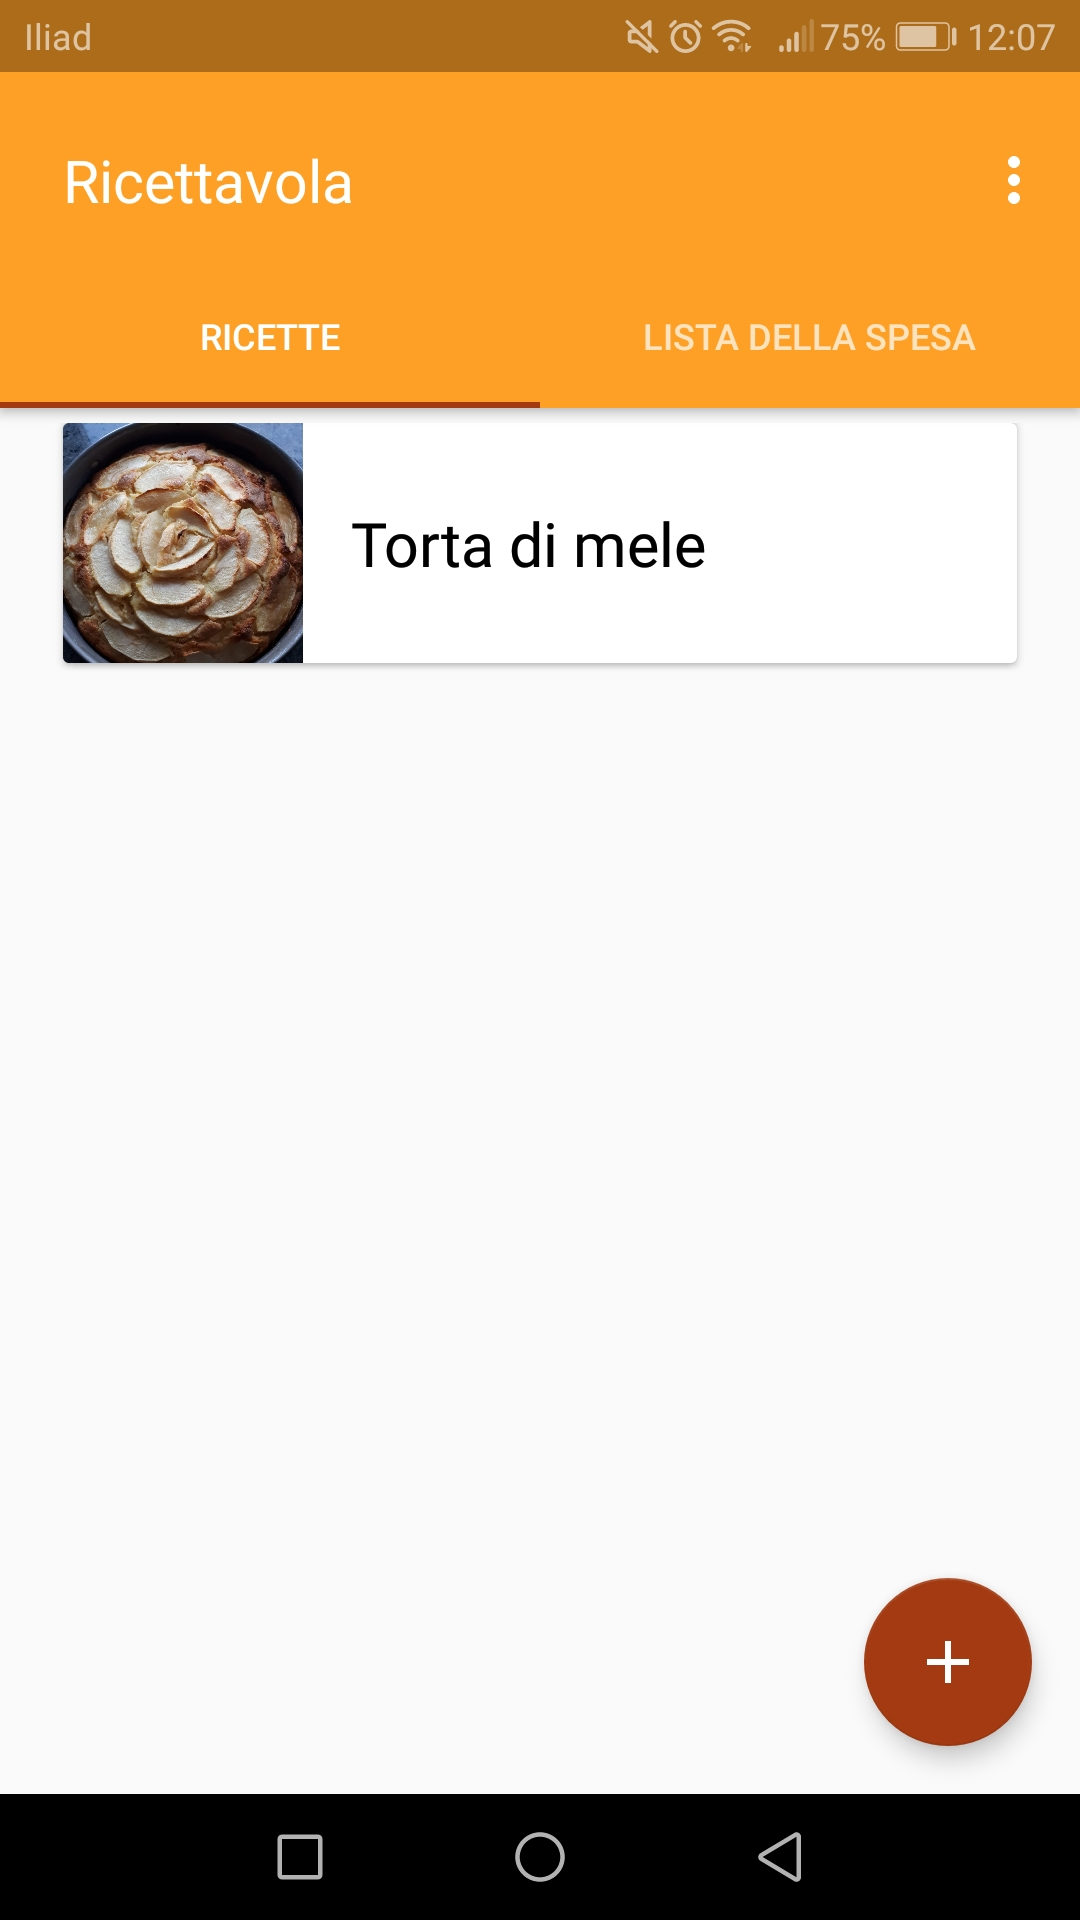
\includegraphics[width=0.5\textwidth]{definitivo/main}
%    & 
%    \vspace{0pt}
%    La schermata principale si presenta come quella progettata durante la prototipizzazione.
%    I tab permettono di spostarti tra le ricette e la lista della spesa.
%    \\
%\end{tabular}



\section{Risultato}
In figura \ref{fig:def_main} è riportata le schermata principale.
Si può notare che la lista delle ricette non presenta differenze rispetto al prototipo a bassa fedeltà.
La lista della spesa invece non è suddivisa per ricette, spetterà all'utente assicurarsi se gli ingredienti ripetuti sono stati ripetuti volutamente o per errore.
Gli ingredienti possono essere selezionati o deselezionati.

\begin{figure}[ht]
  \begin{center}
    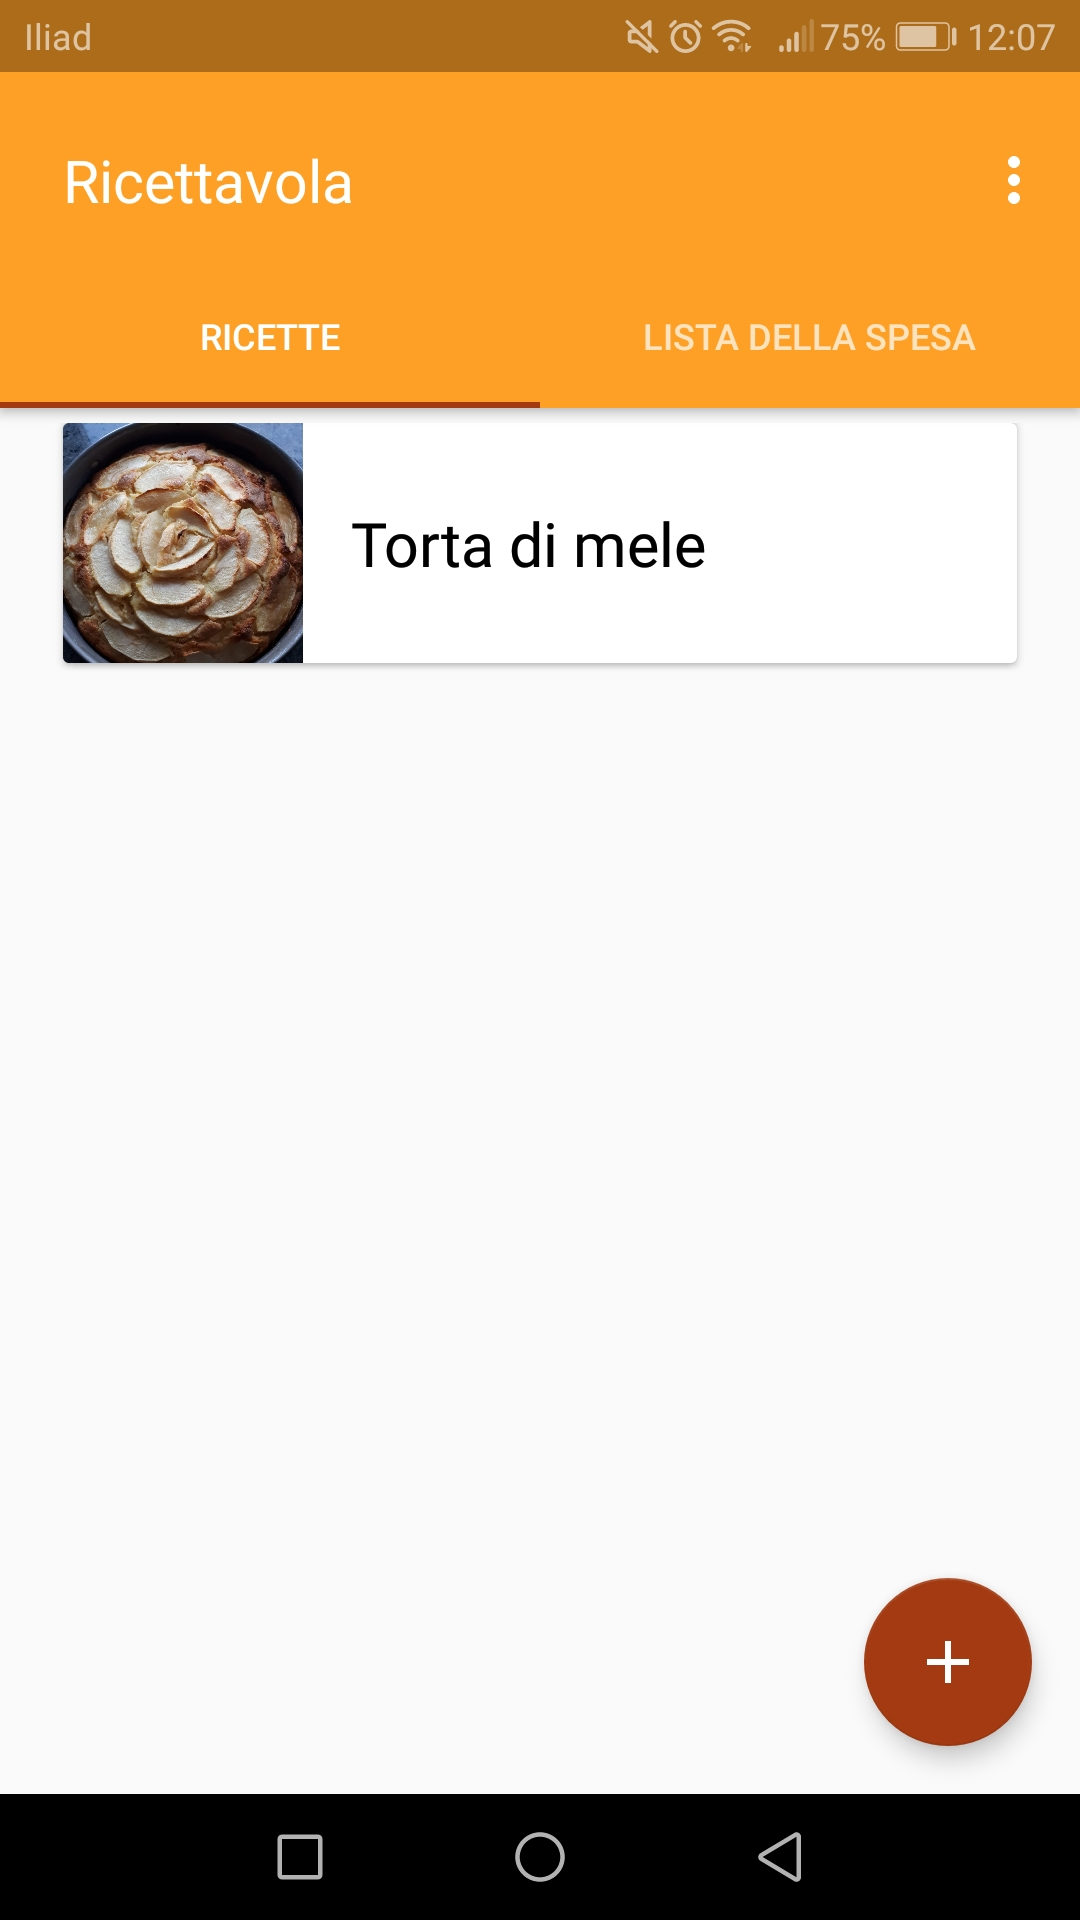
\includegraphics[width=0.49\textwidth]{definitivo/main}
    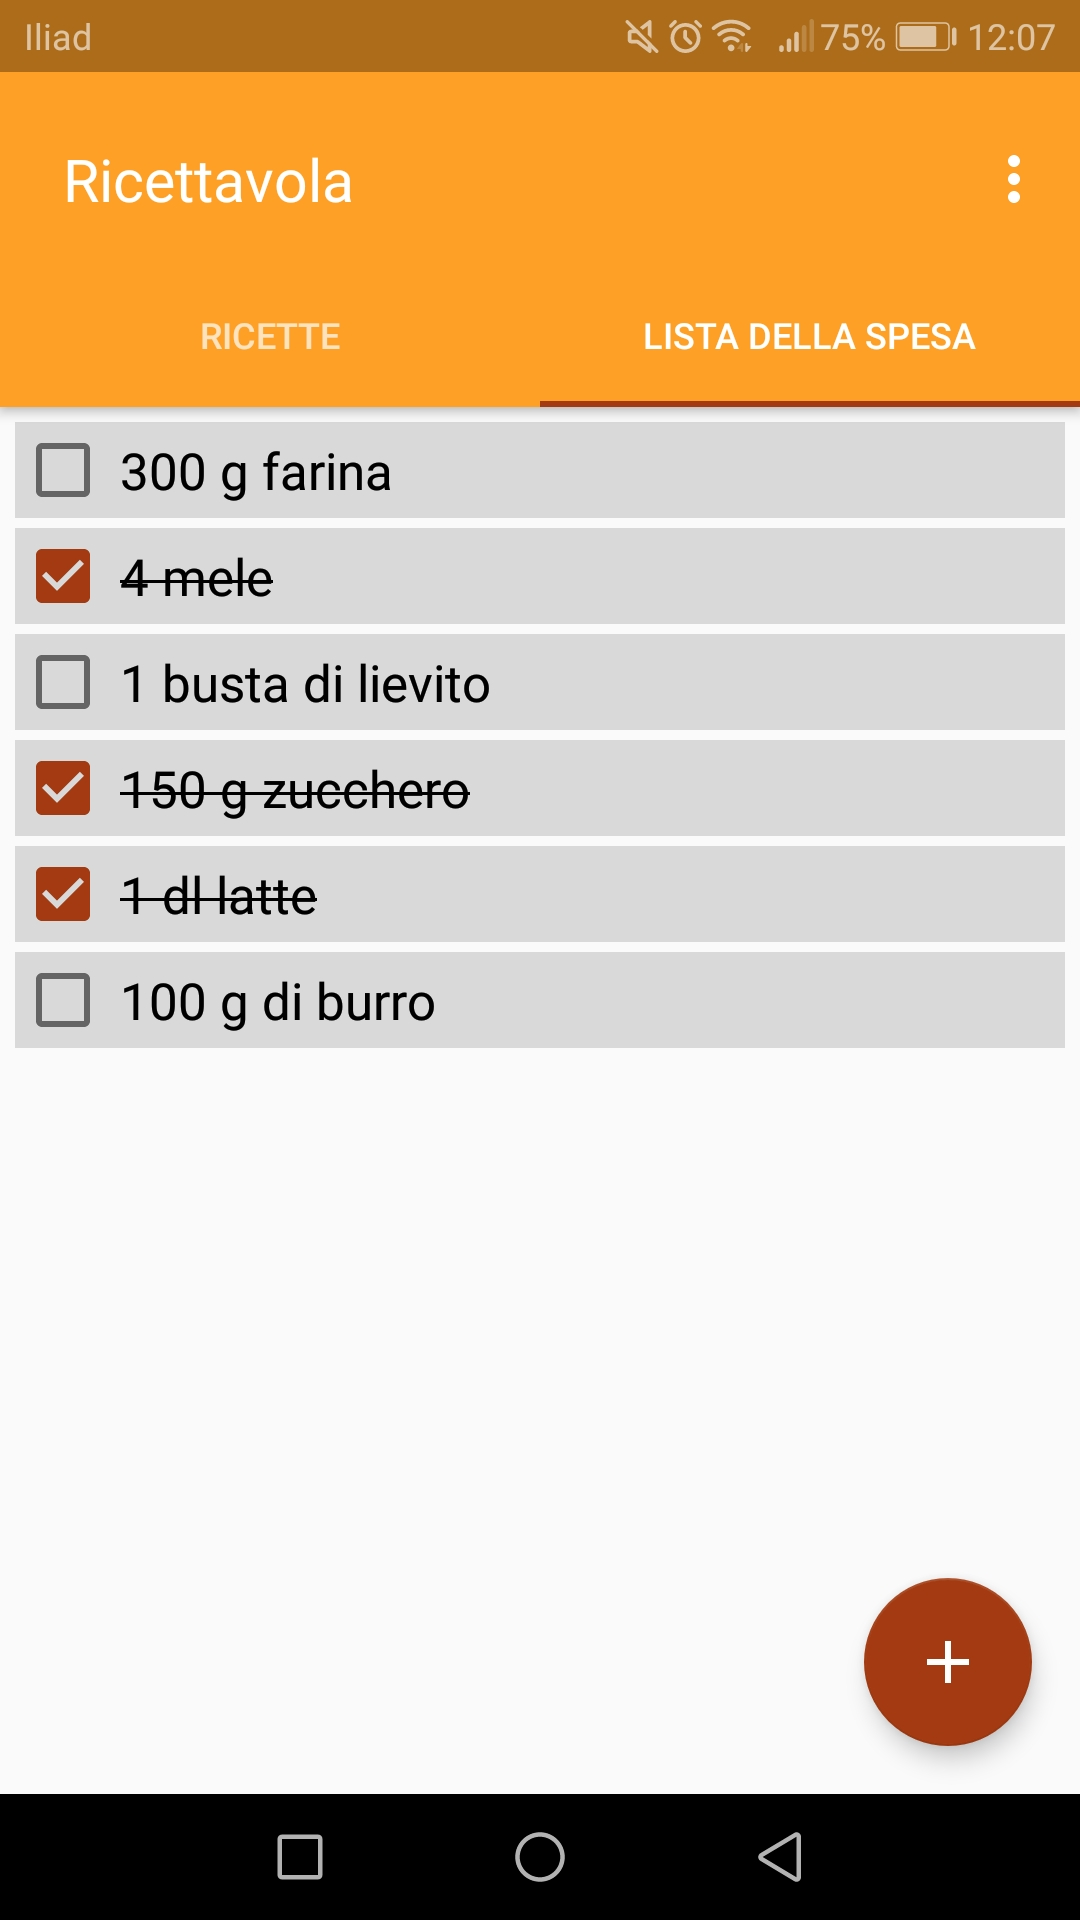
\includegraphics[width=0.49\textwidth]{definitivo/lista_della_spesa}
    \caption{Schermata principale}
    \label{fig:def_main}
  \end{center}
\end{figure}

Tendo premuto su una ricetta è possibile far comparire un cestino per ogni elemento.
Se l'icona viene premuta compare una messaggio come quello in figura \ref{fig:def_main_3}.
Notare che le due immagini corrispondono allo stesso messaggio, ma nel secondo la lingua dell'applicazione è impostata sull'inglese.

\begin{figure}[ht]
  \begin{center}
    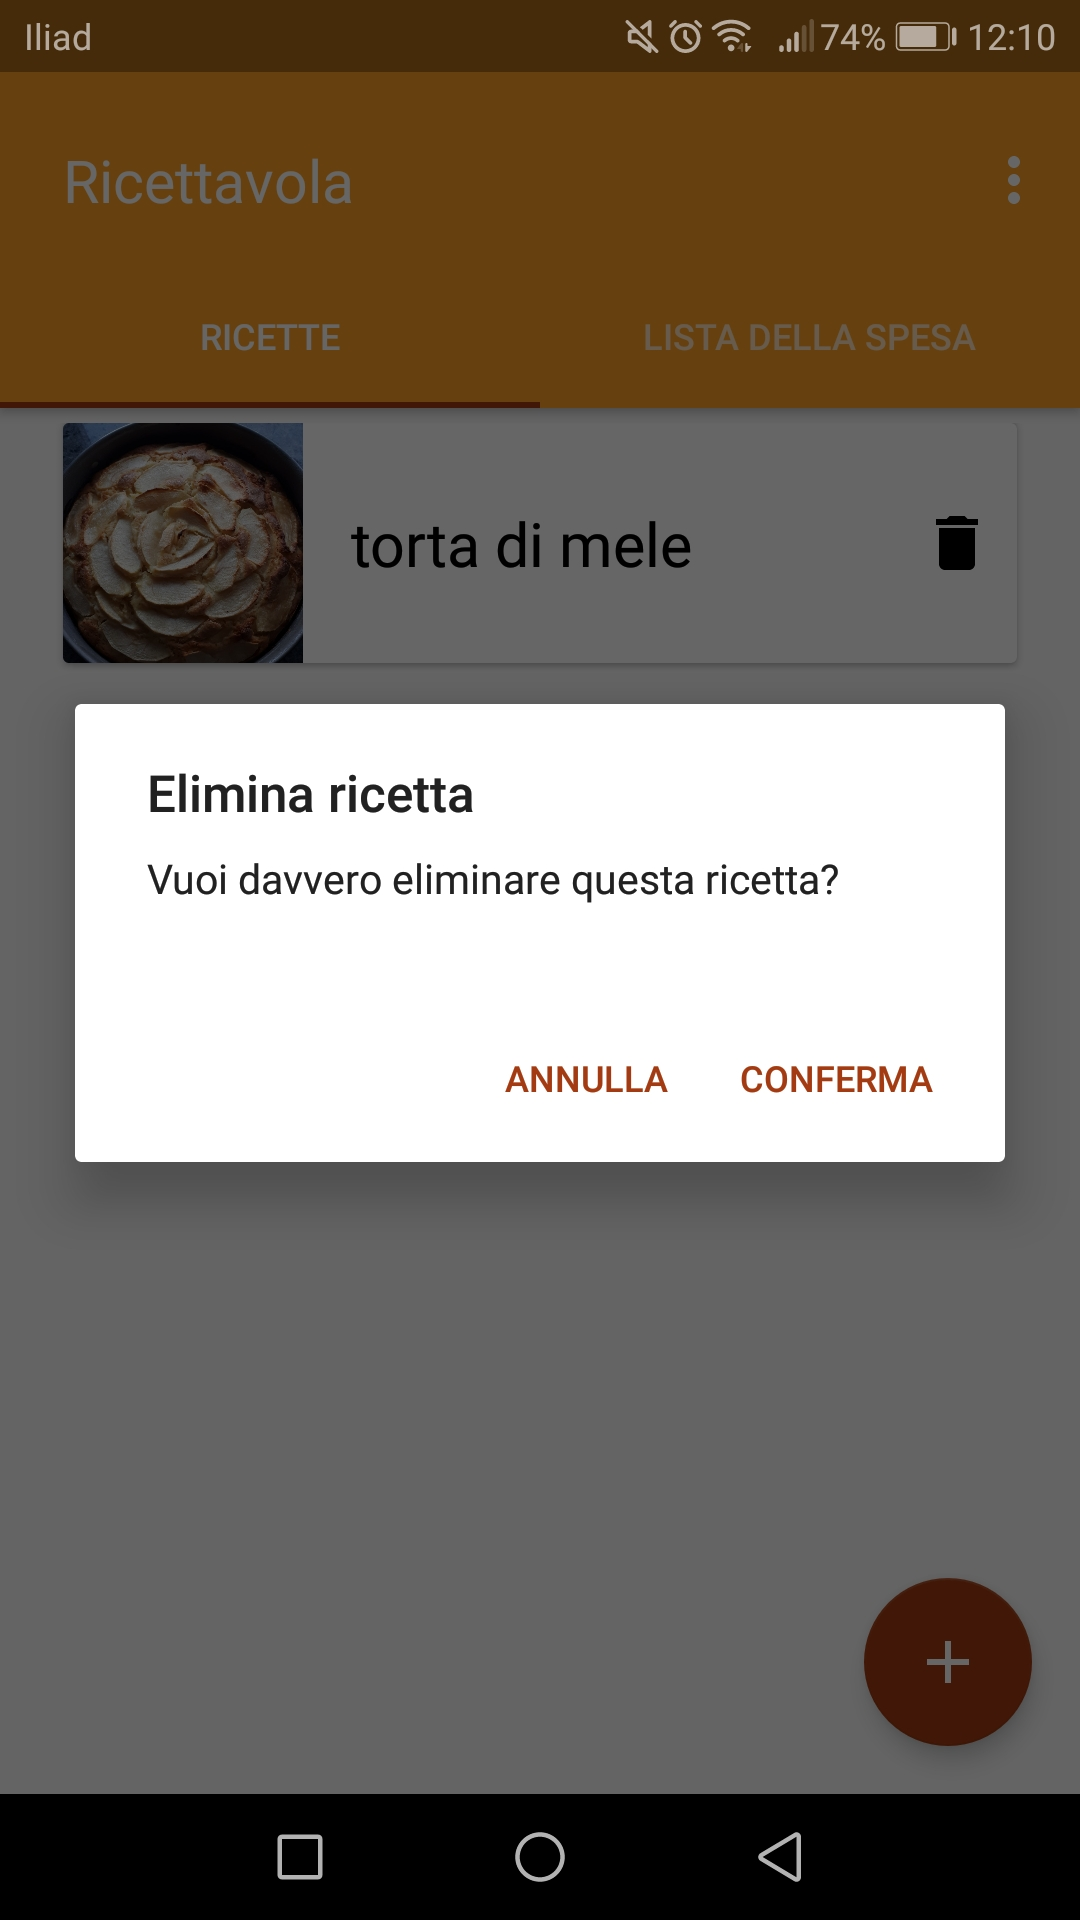
\includegraphics[width=0.49\textwidth]{definitivo/elimina_ricetta}
    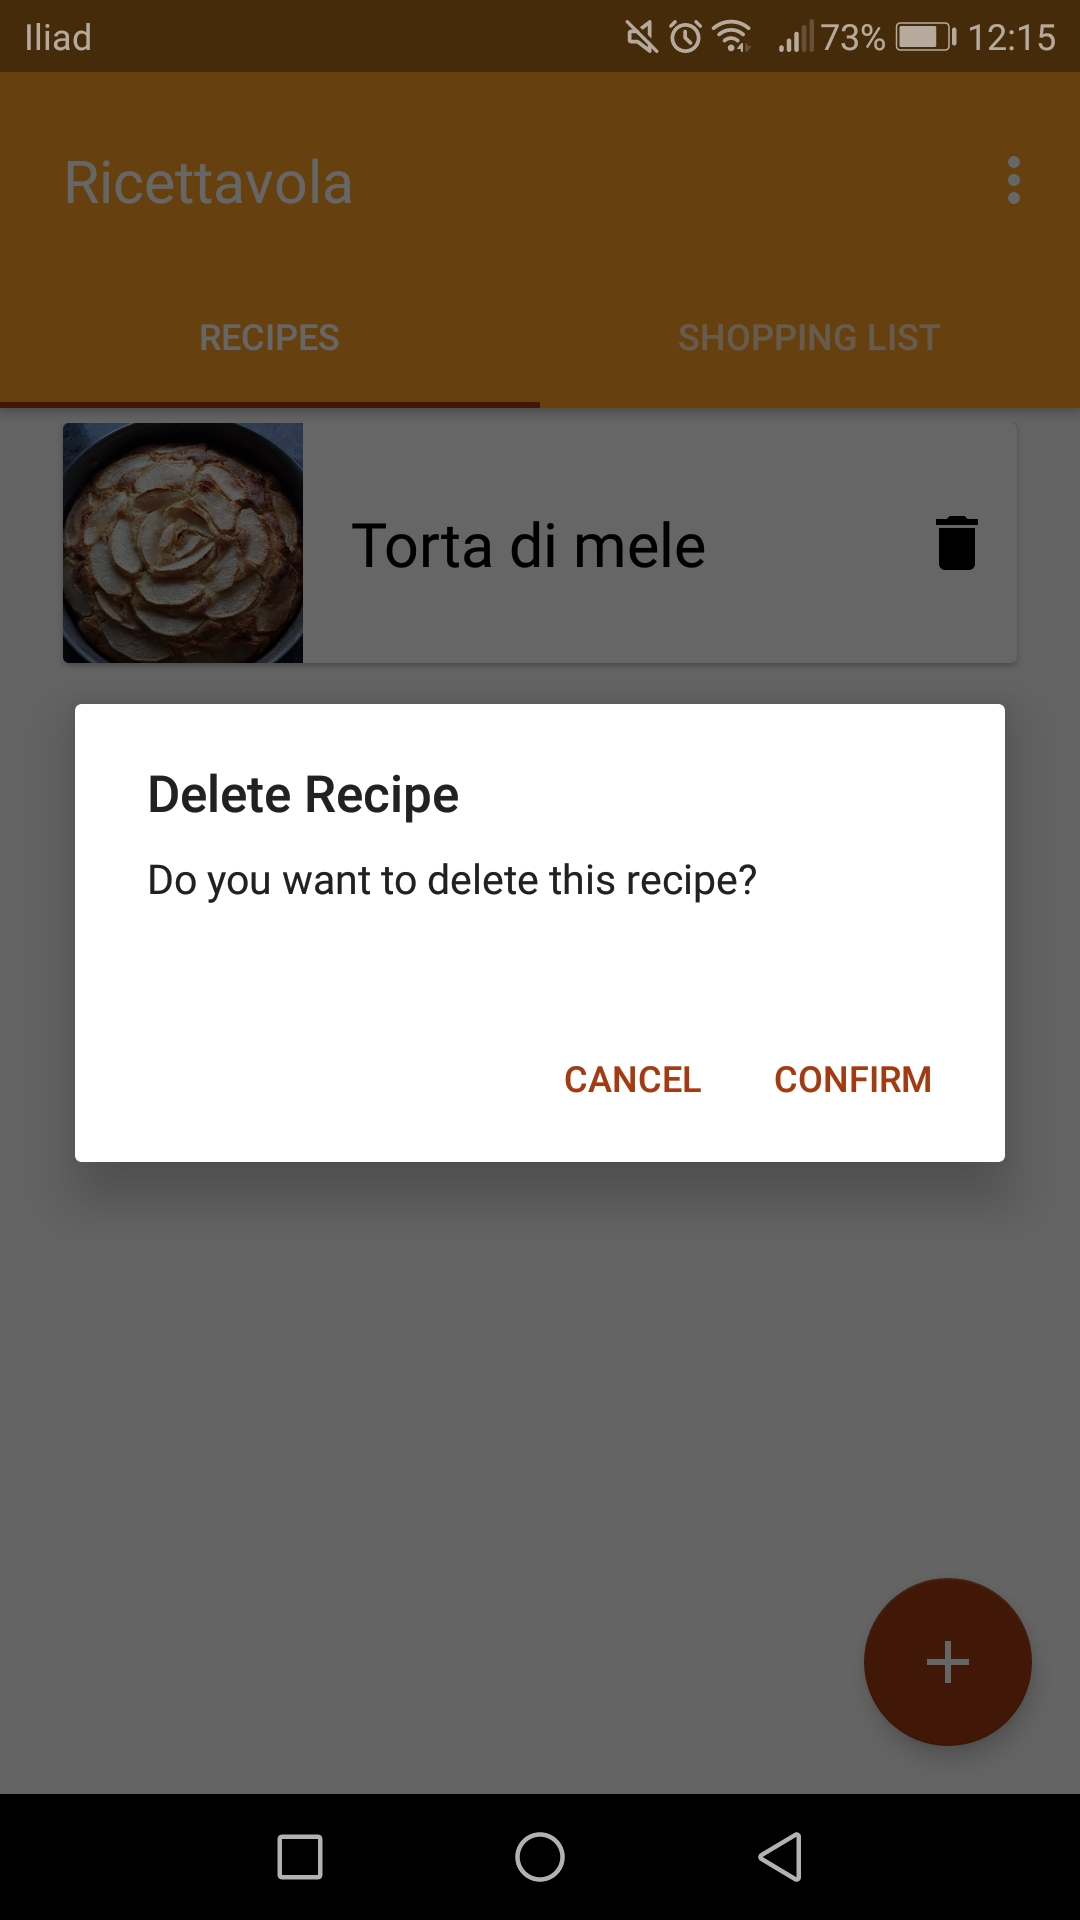
\includegraphics[width=0.49\textwidth]{definitivo/elimina_ricetta_eng}
    \caption{Messaggio di conferma eliminazione ricetta}
    \label{fig:def_main_3}
  \end{center}
\end{figure}

In figura \ref{fig:def_main_2} è illustrato il menù a tendina dell'attività principale.
L'ultima voce, a prescindere dalla lingua, riporta "Change language" così la sua funzione rimane chiara indipendentemente dalla lingua attuale.
Premendo questa voce si può passare a rotazione tra lingue italiano ed inglese.
Appena sopra sono presenti due voci per la manipolazione della lista della spesa.
Premendo "Aggiungi ricetta da clipboard" verrà verificato se il testo nella \textit{clipboard} corrisponde a quello di una ricetta.
In caso affermativo la ricetta apparirà nell'elenco delle ricette, altrimenti comparirà un messaggio d'errore.

\begin{figure}[ht]
  \begin{center}
    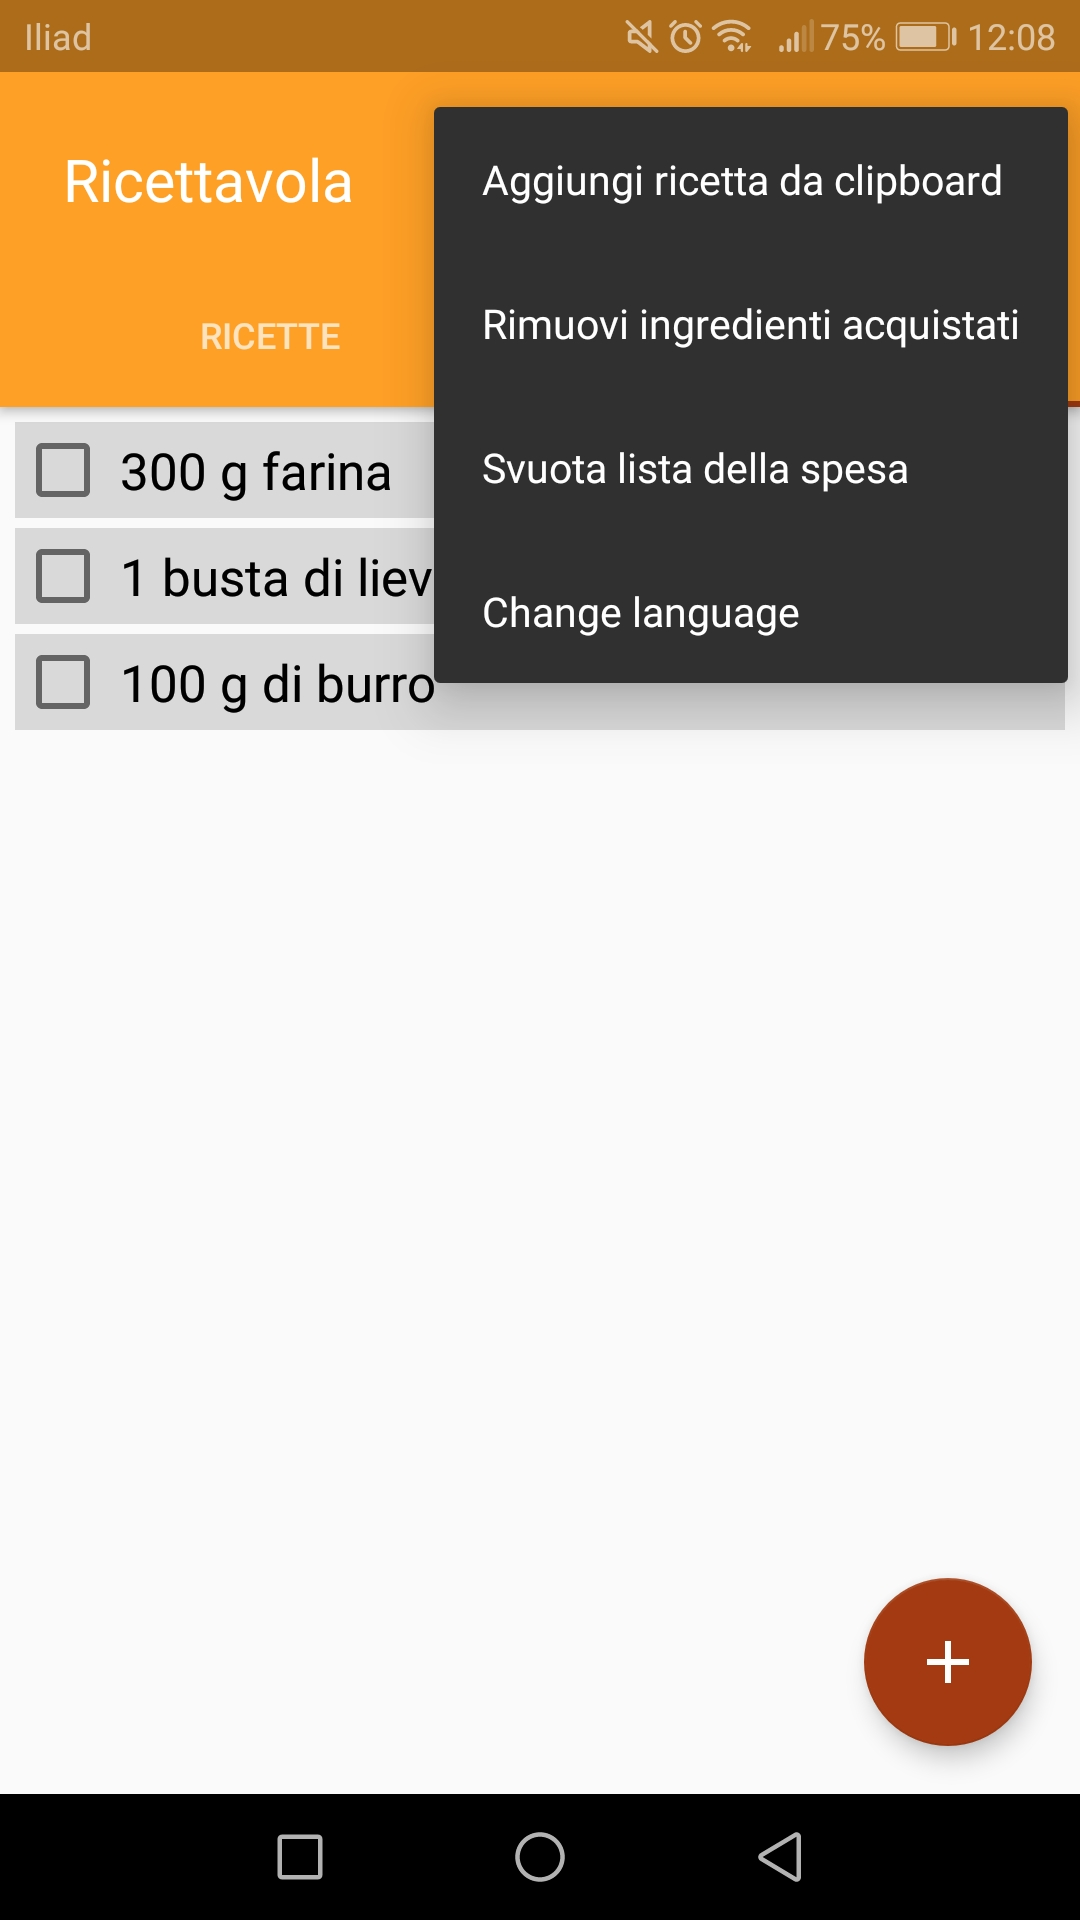
\includegraphics[width=0.8\textwidth]{definitivo/menu_main}
    \caption{Menù schermata principale}
    \label{fig:def_main_2}
  \end{center}
\end{figure}
\clearpage

Premendo il tasto per aggiungere una ricetta verrà mostrata la schermata in figura \ref{fig:def_nuova}.
\begin{figure}[ht]
  \begin{center}
    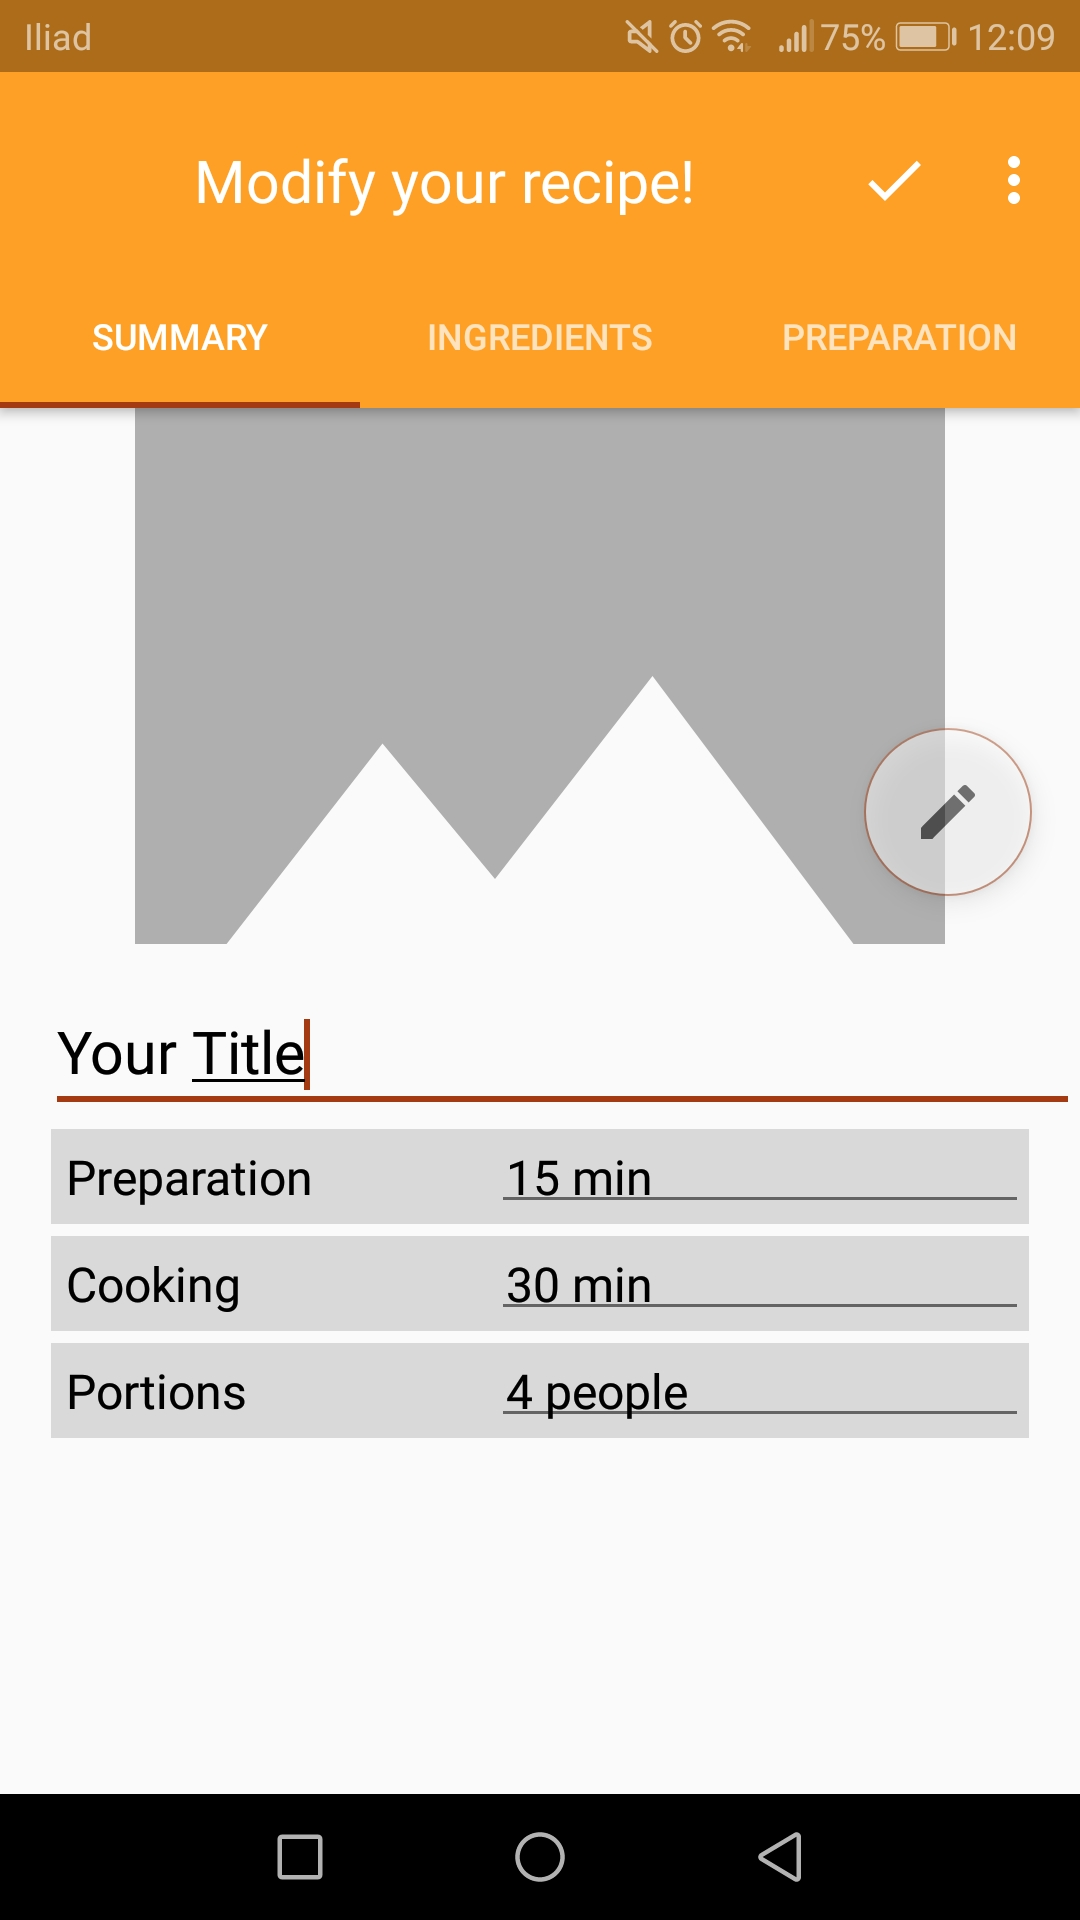
\includegraphics[width=0.6\textwidth]{definitivo/nuova_ricetta_eng}
    \caption{Schermata di una nuova ricetta}
    \label{fig:def_nuova}
  \end{center}
\end{figure}

\begin{figure}[ht]
  \begin{center}
    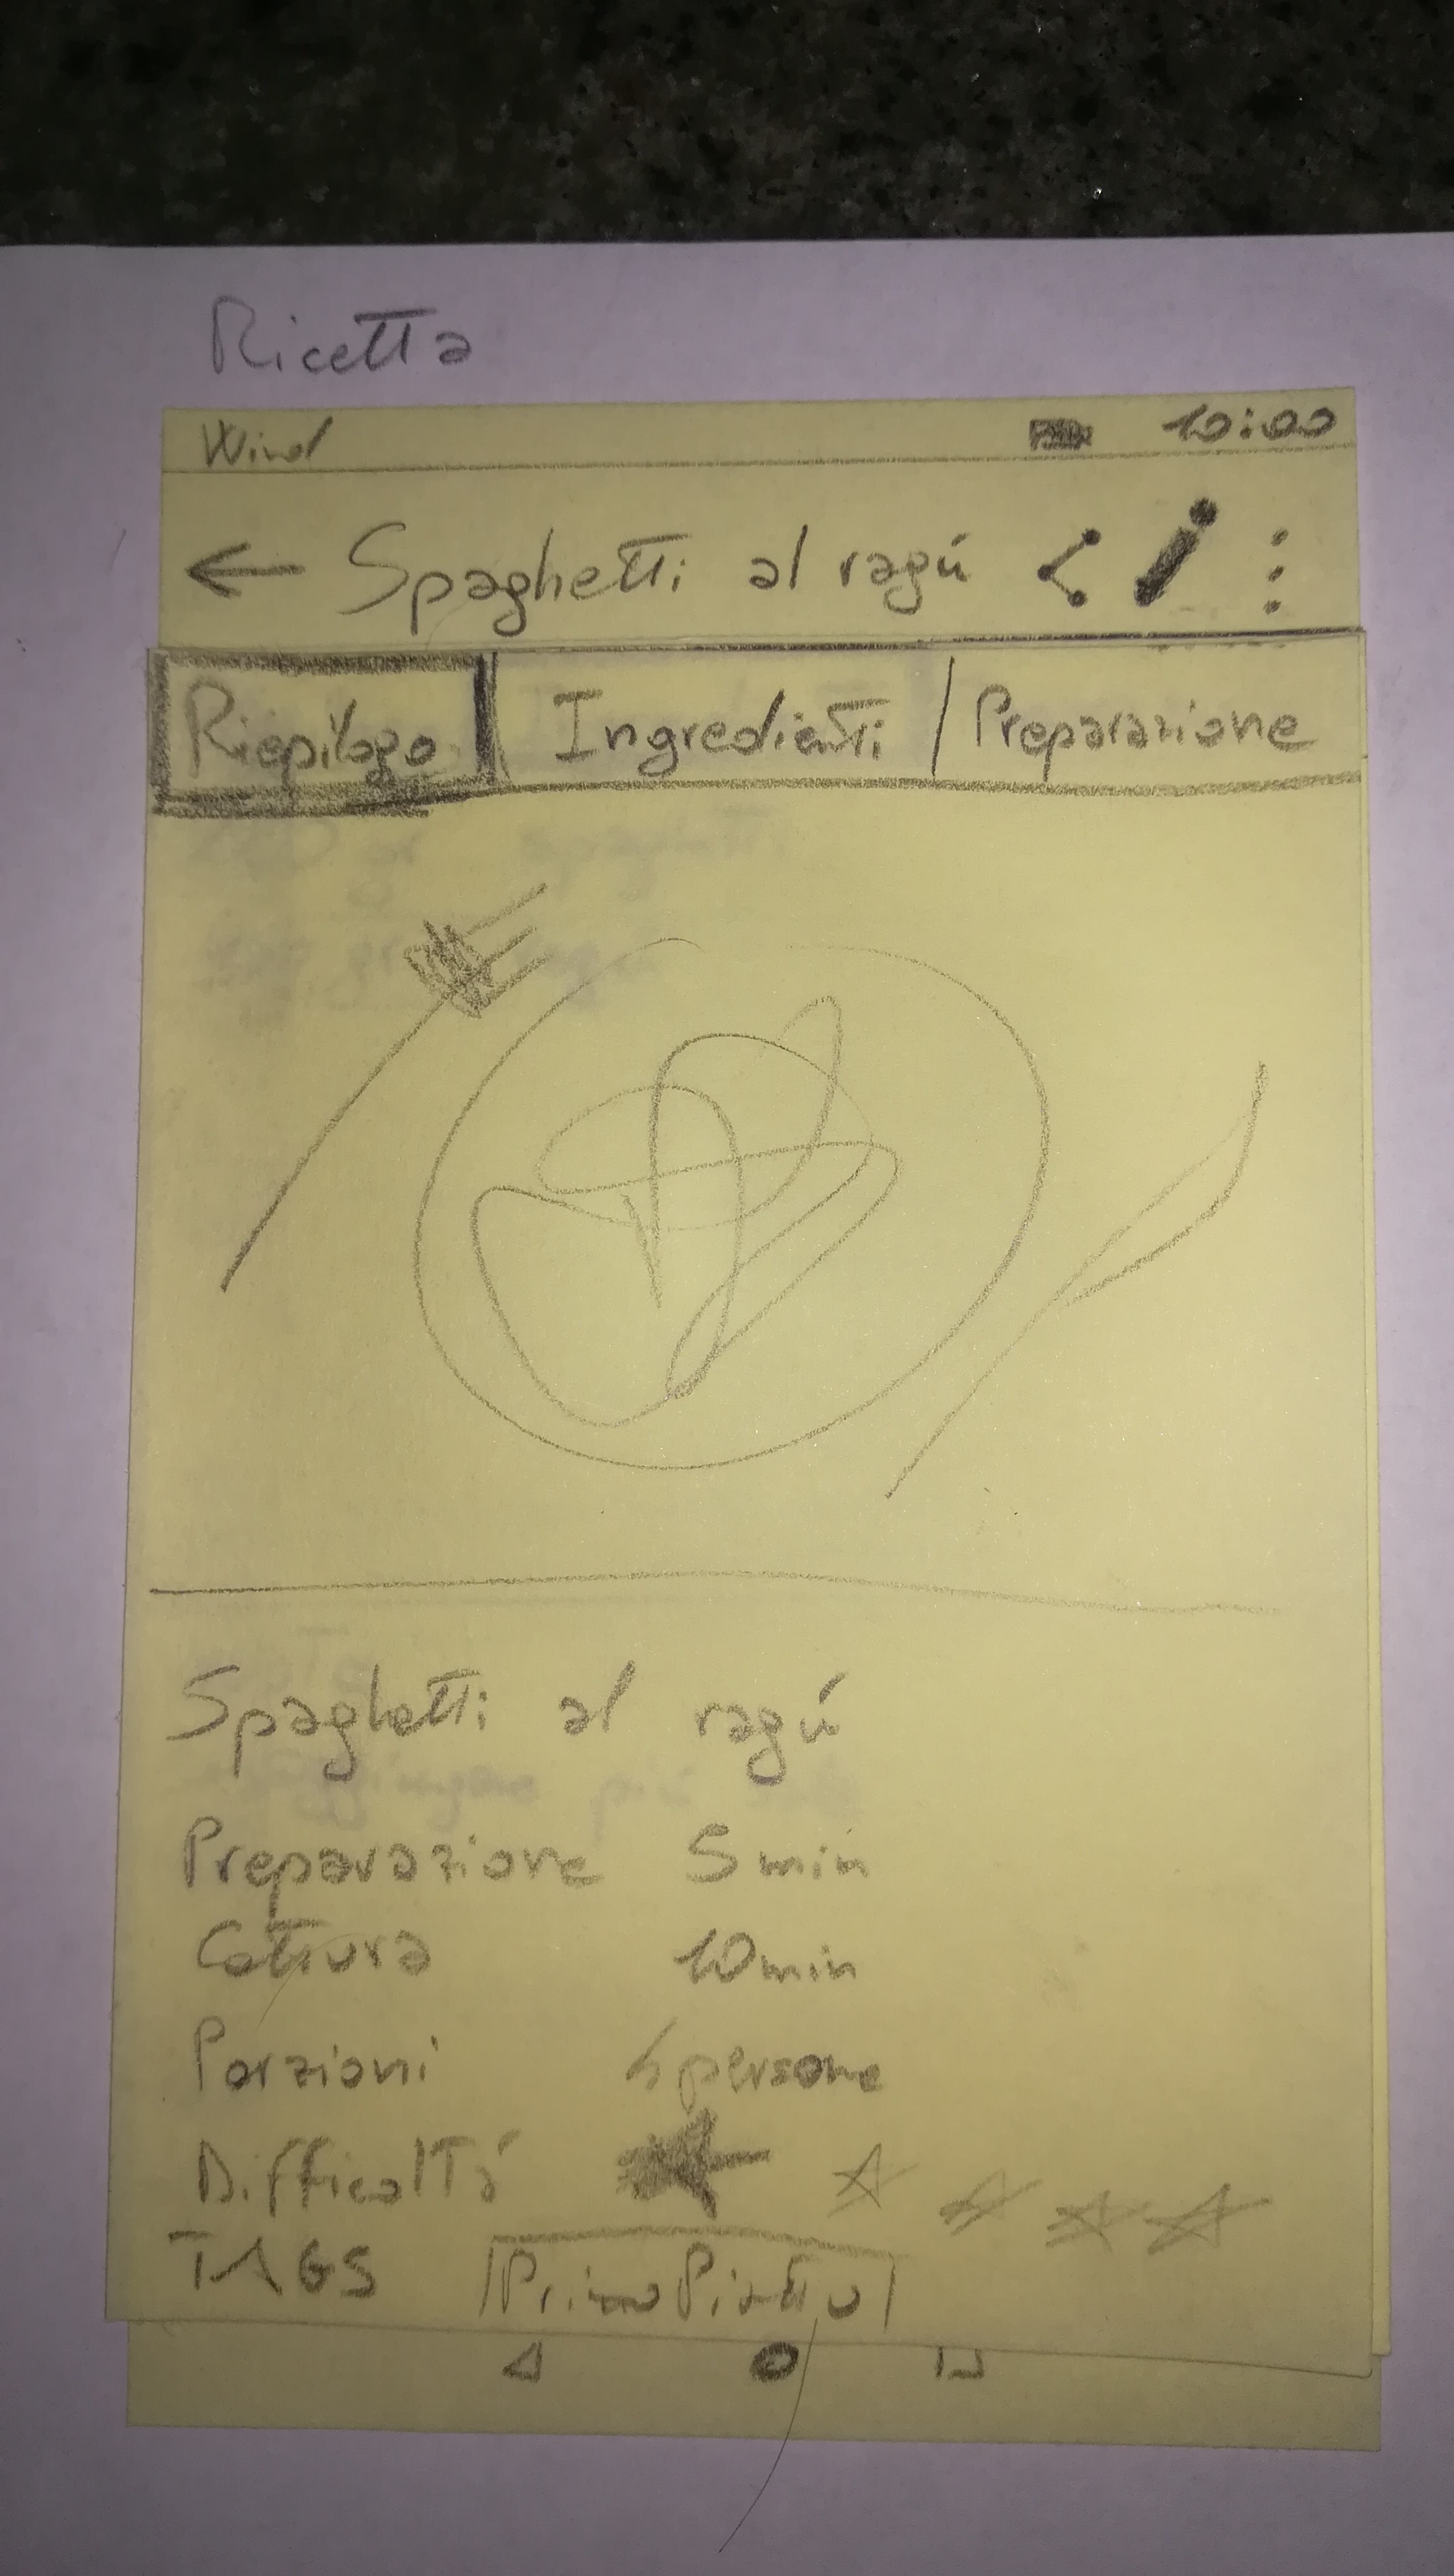
\includegraphics[width=0.49\textwidth]{definitivo/ricetta_riepilogo}
    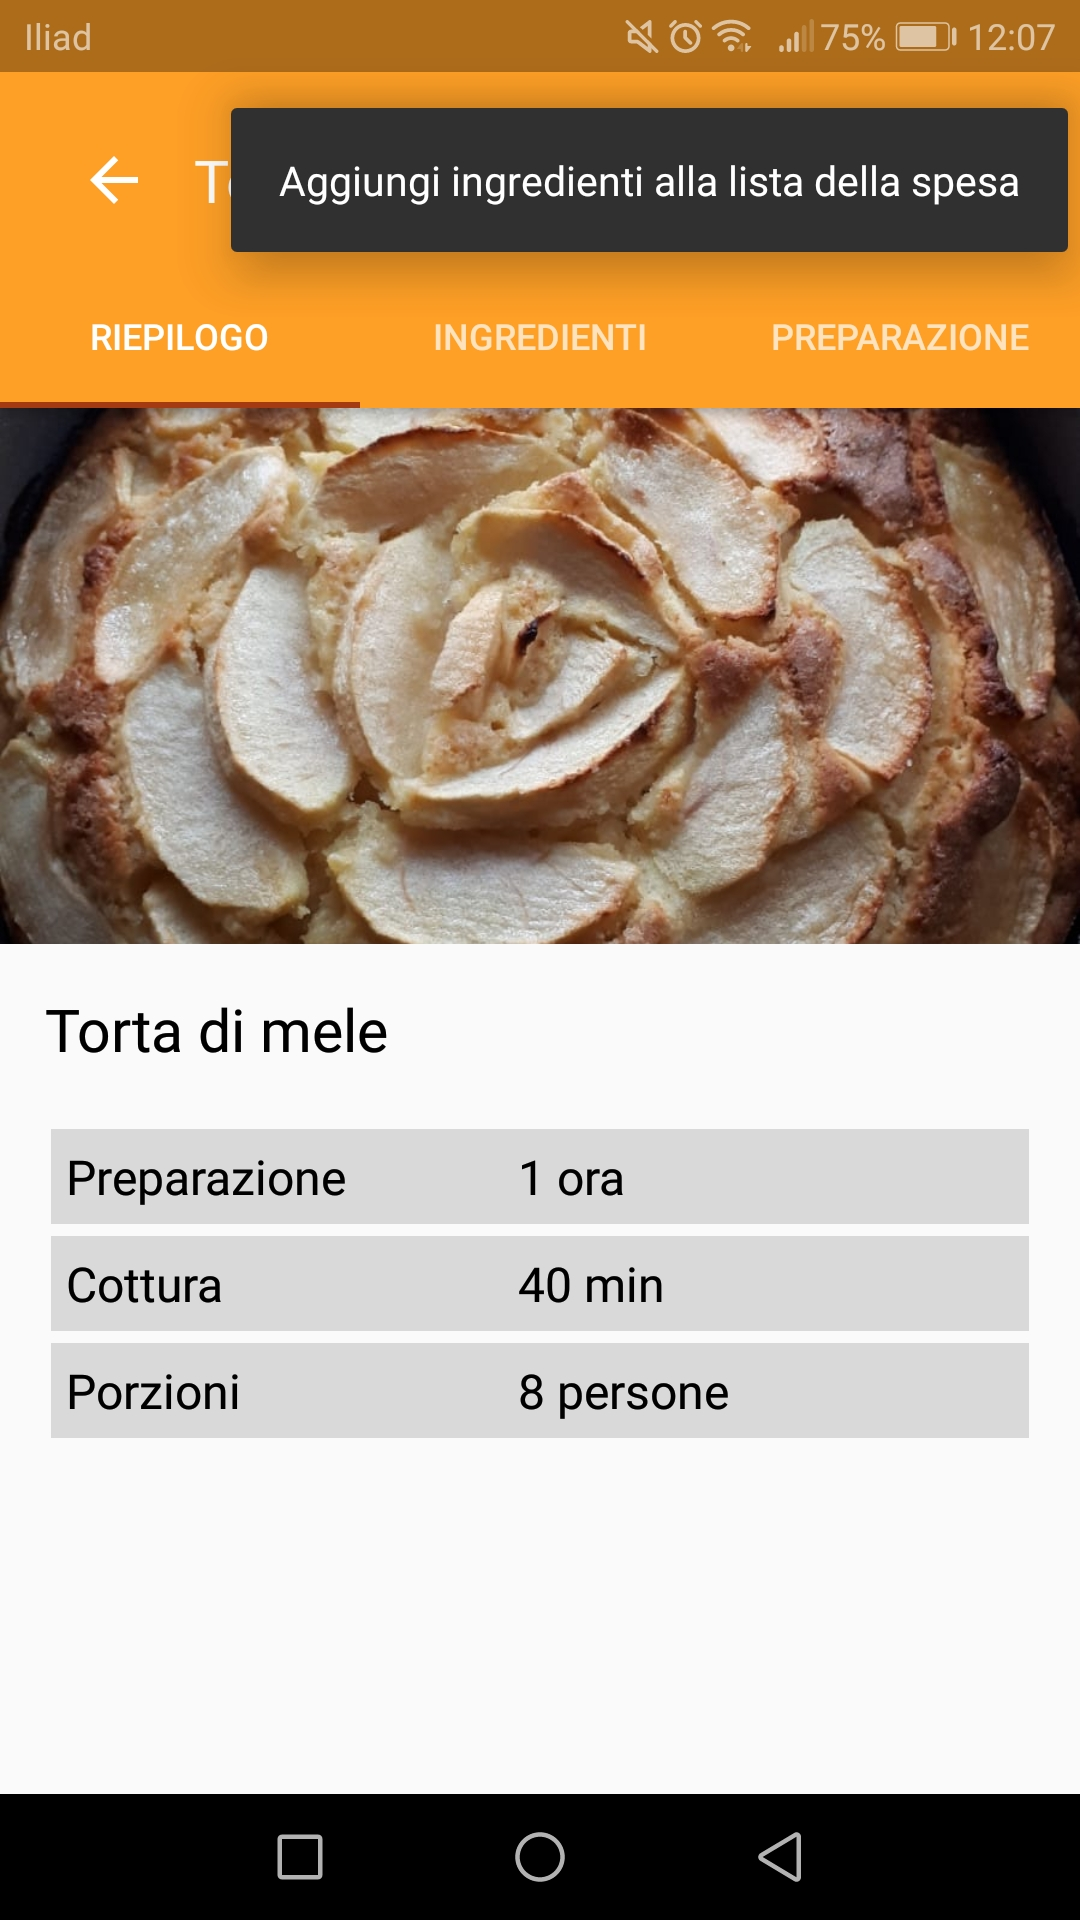
\includegraphics[width=0.49\textwidth]{definitivo/menu_riepilogo}
    \caption{Schermata di riepilogo di una ricetta e suo menù}
    \label{fig:def_ricetta}
  \end{center}
\end{figure}

\begin{figure}[ht]
  \begin{center}
    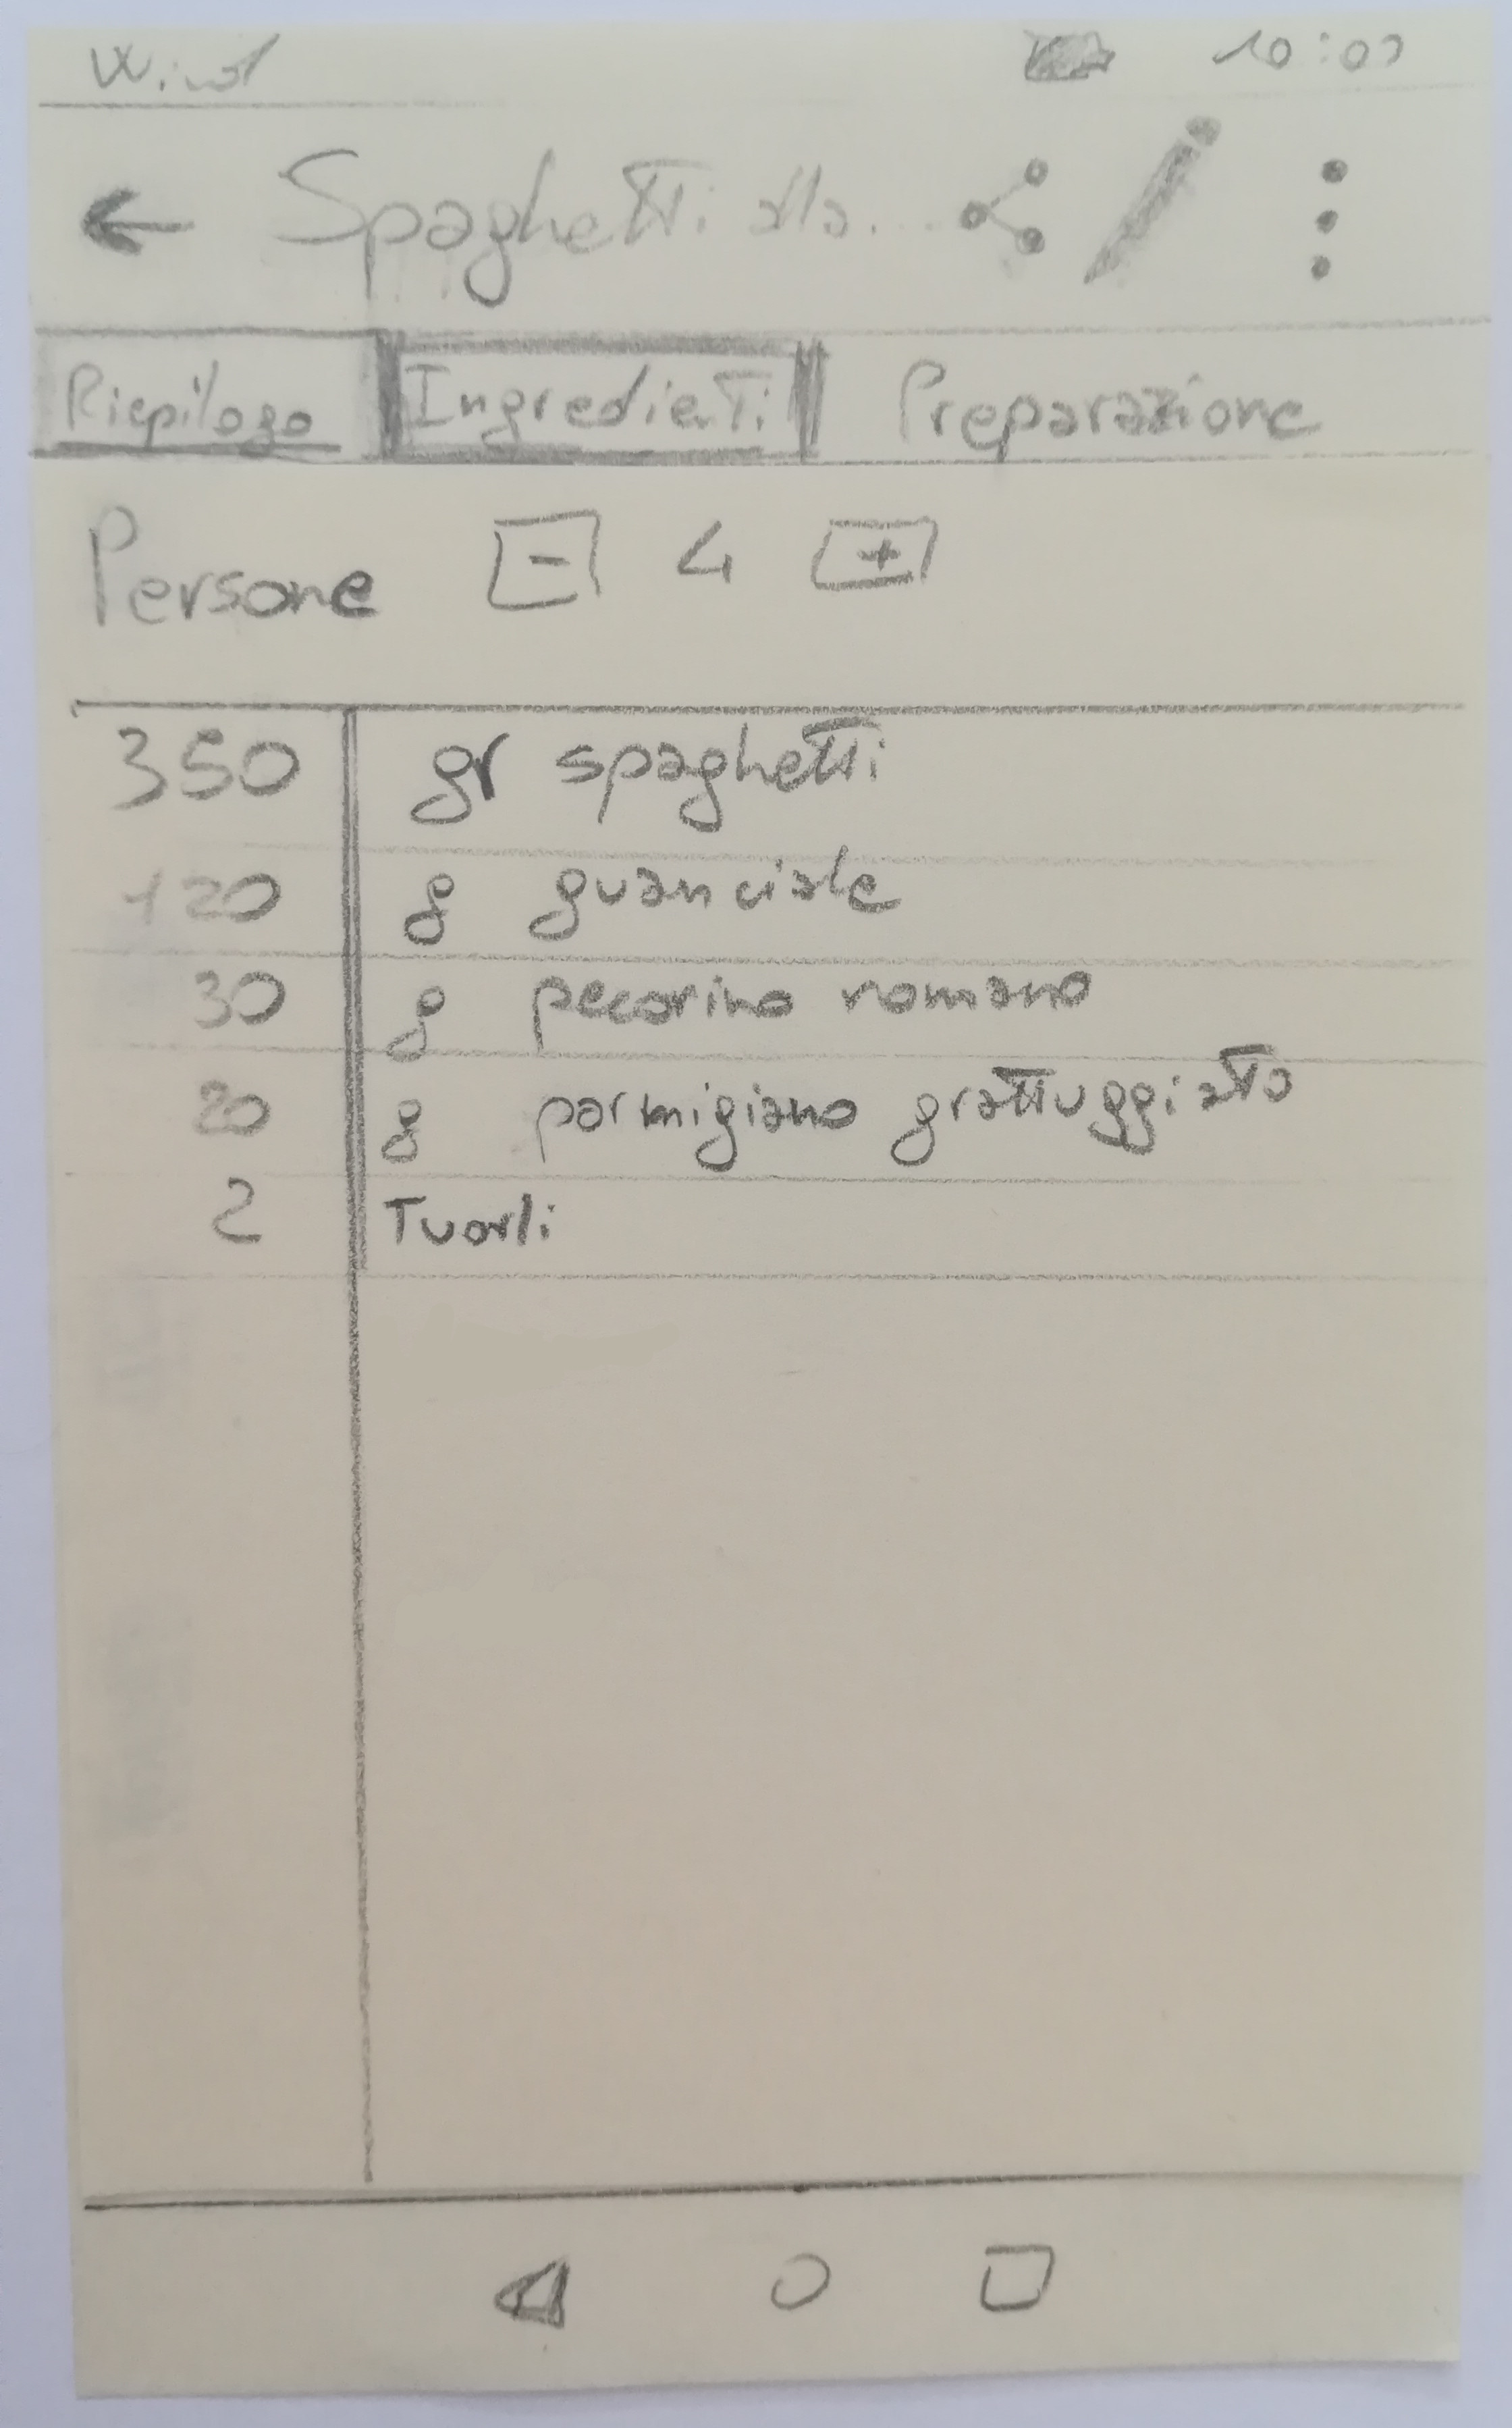
\includegraphics[width=0.49\textwidth]{definitivo/ricetta_ingredienti}
    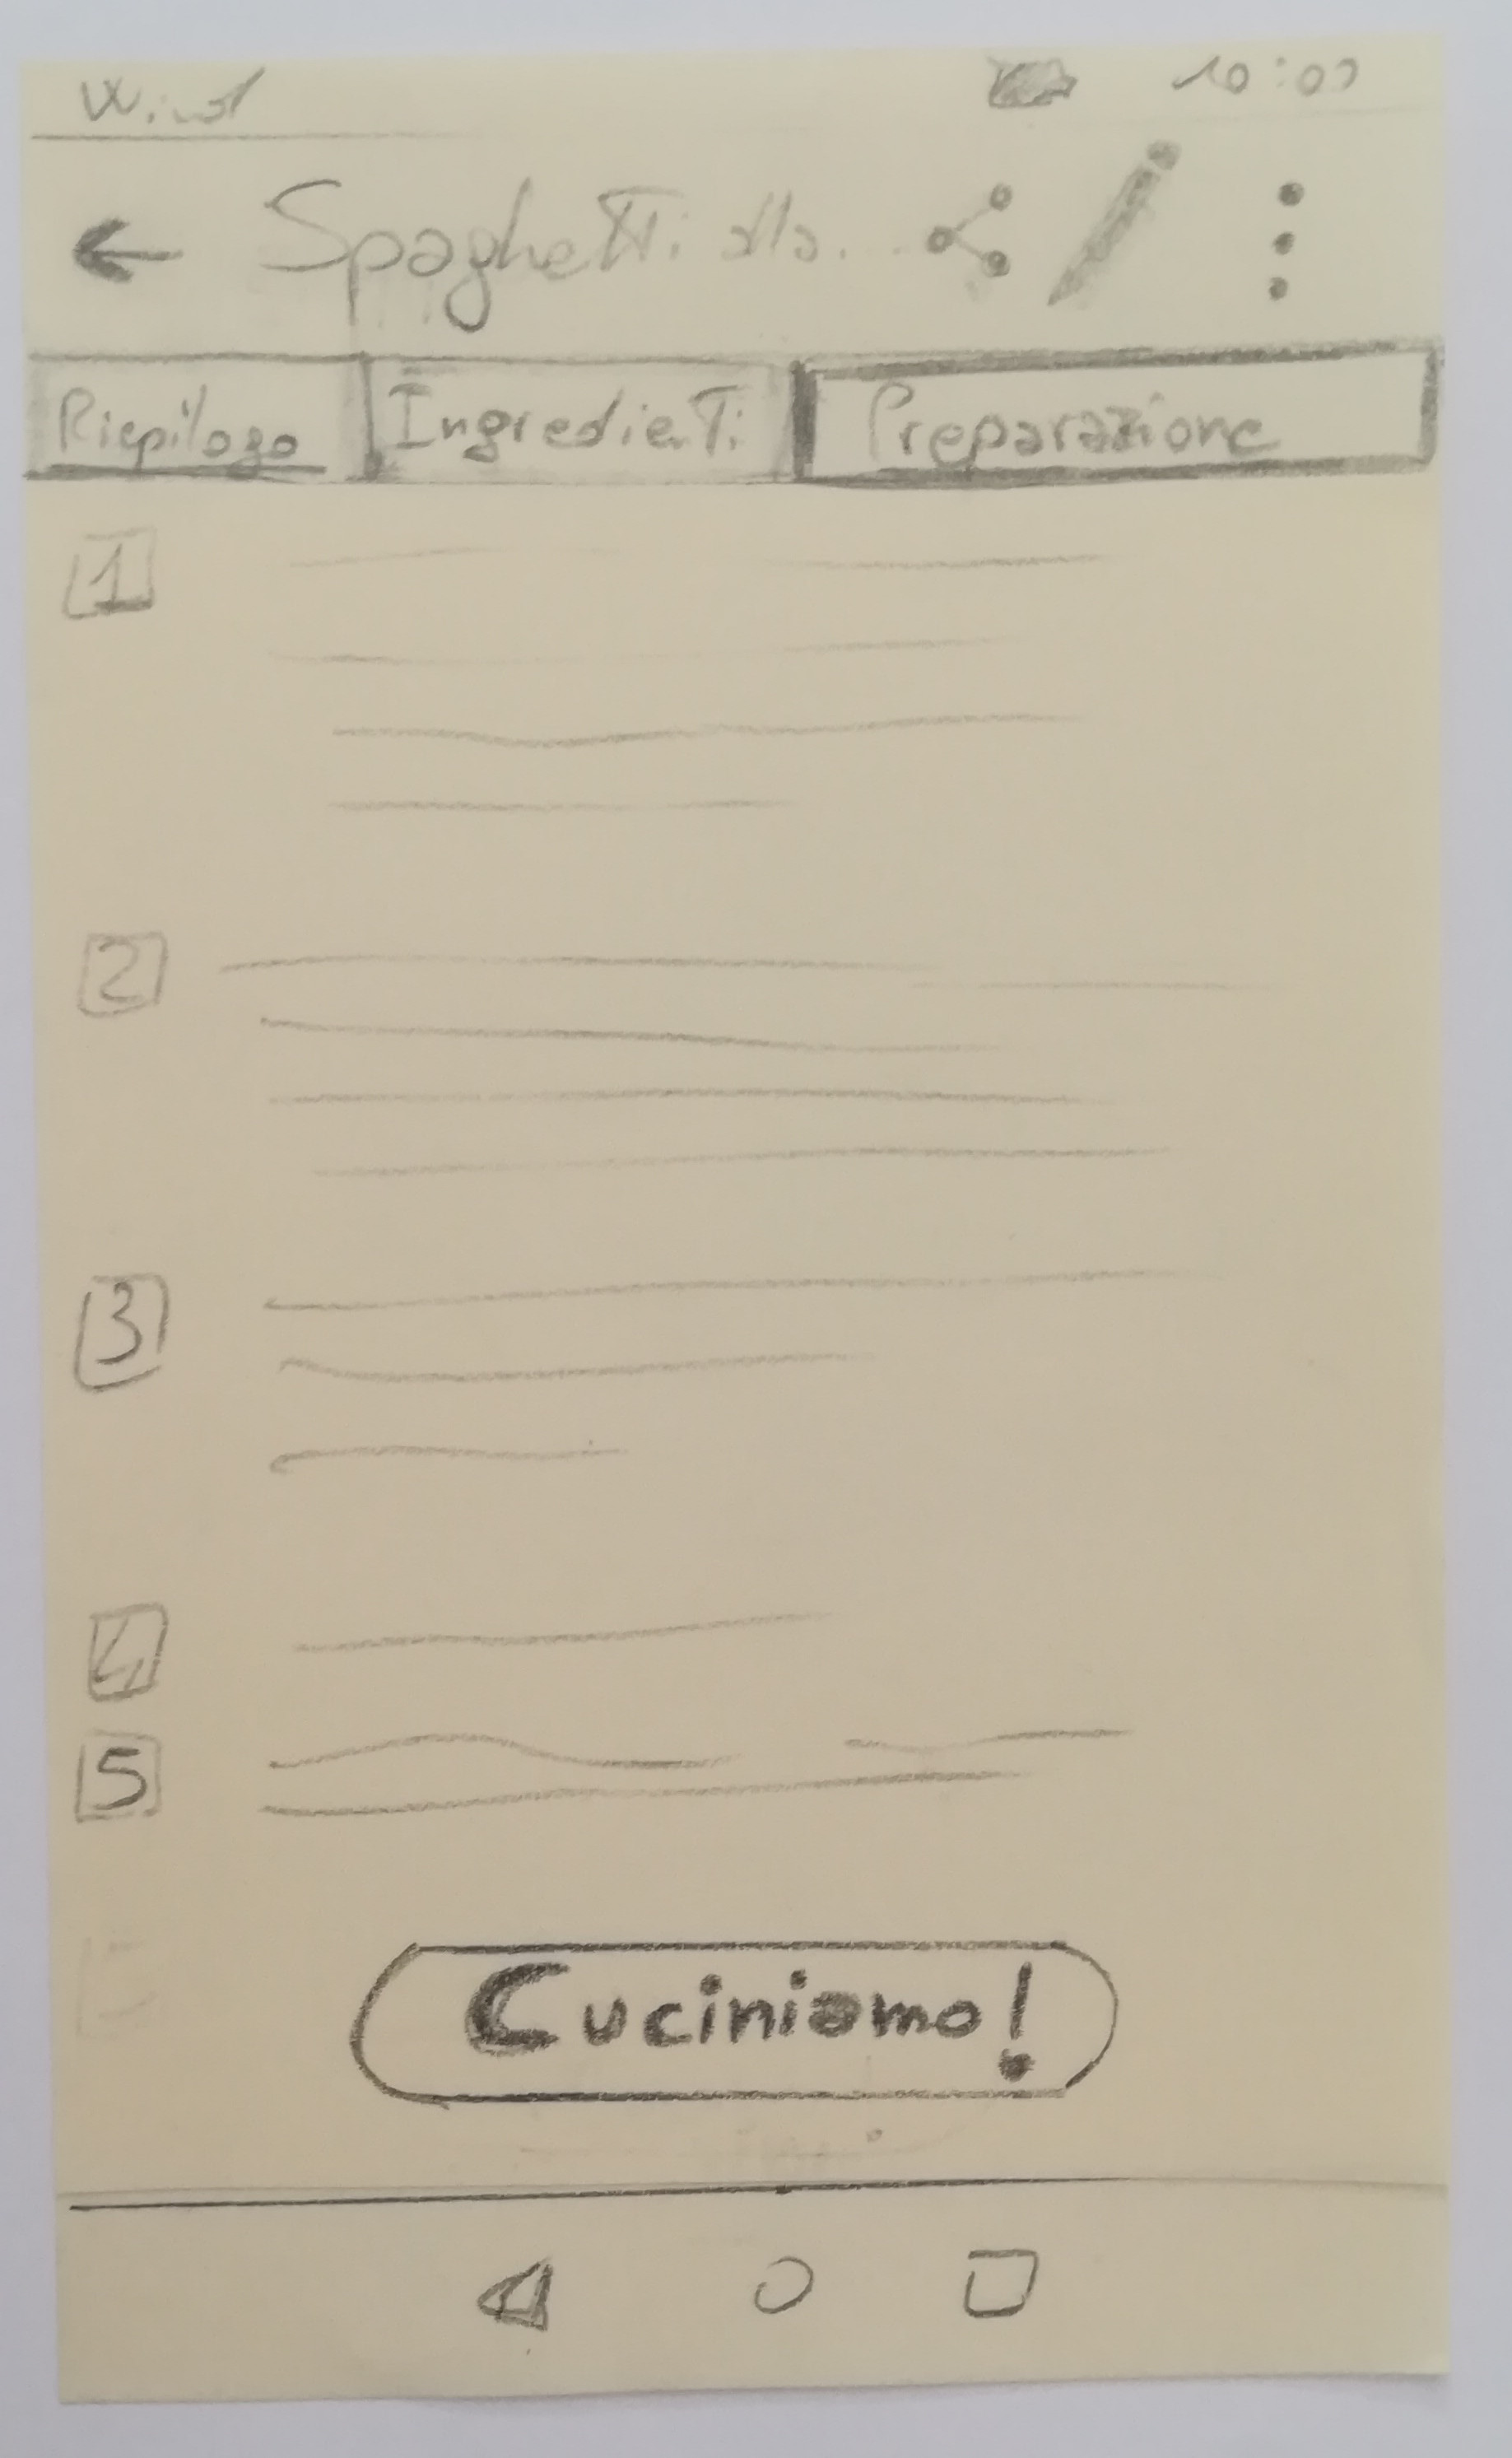
\includegraphics[width=0.49\textwidth]{definitivo/ricetta_preparazione}
    \caption{Schermate ingredienti e preparazione}
    \label{fig:def_ricetta_1}
  \end{center}
\end{figure}

\begin{figure}[ht]
   \begin{center}
    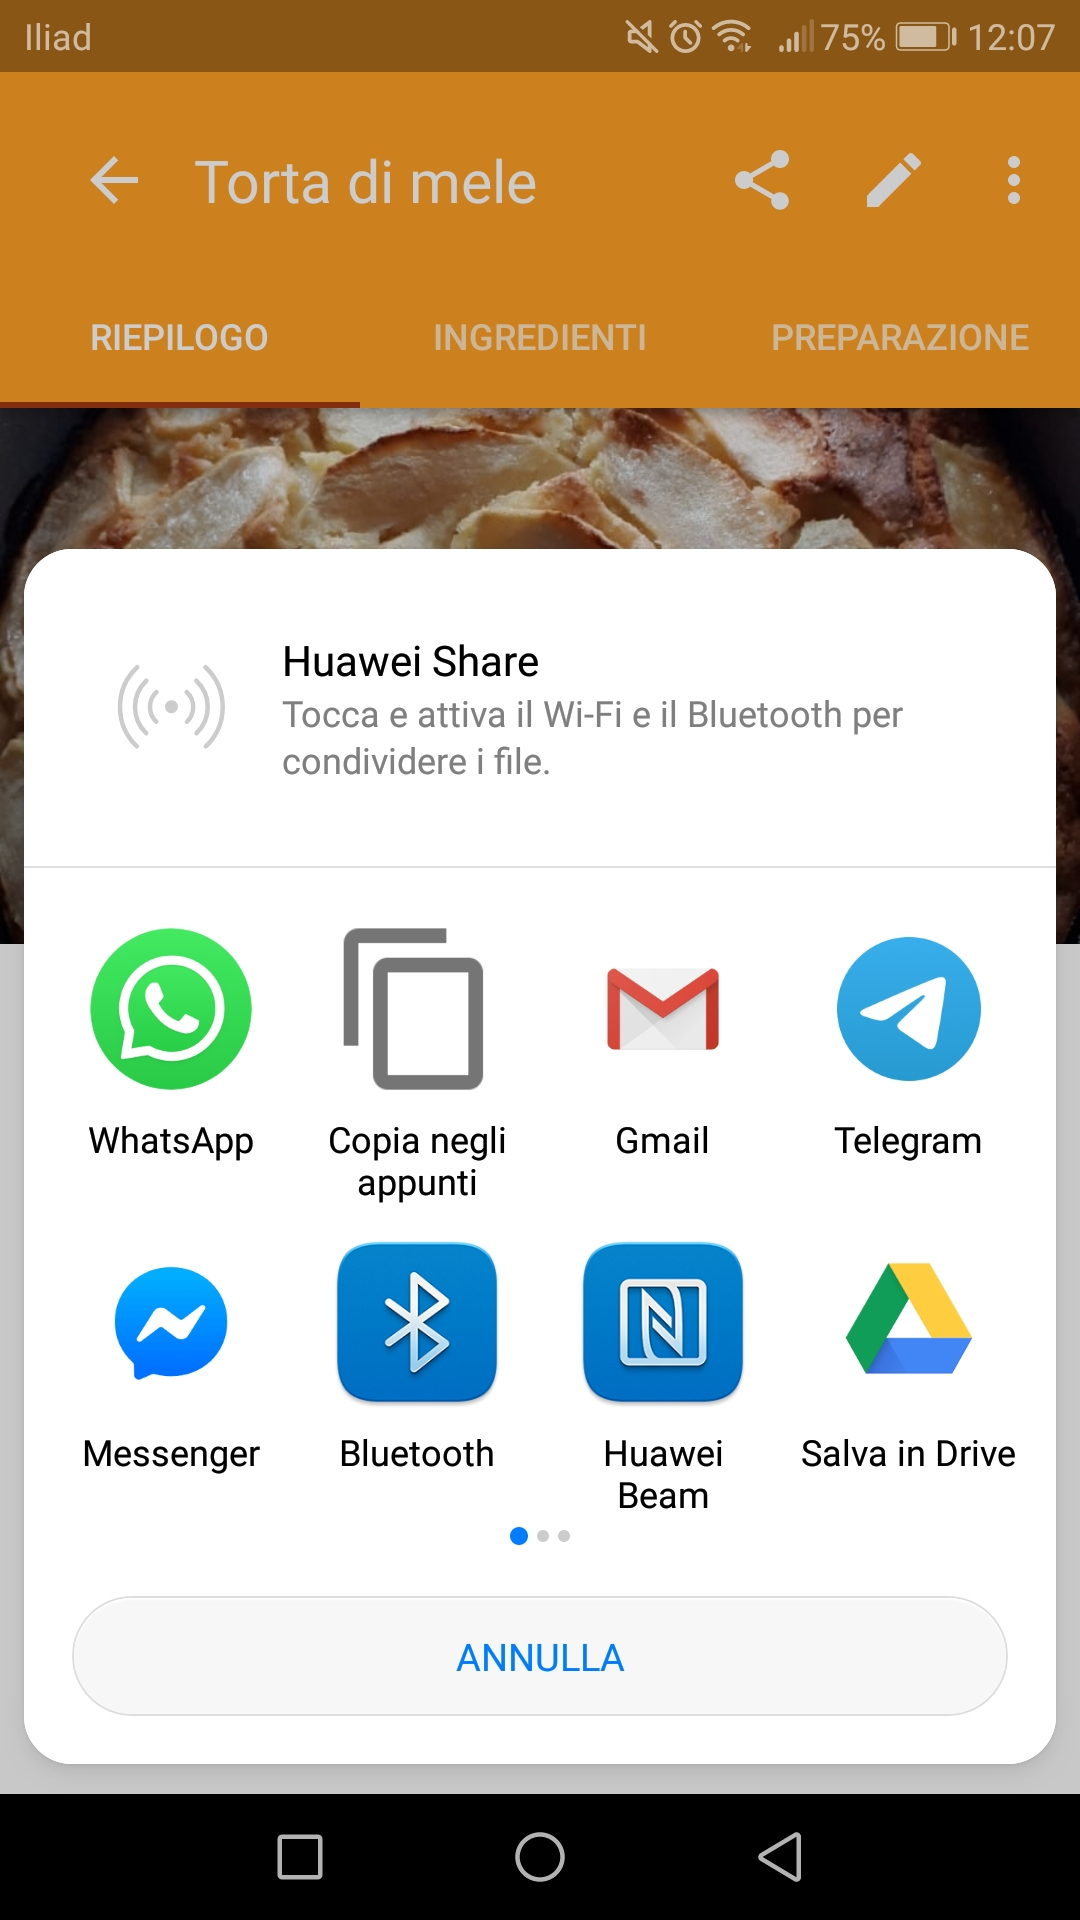
\includegraphics[width=0.49\textwidth]{definitivo/tasto_share}
    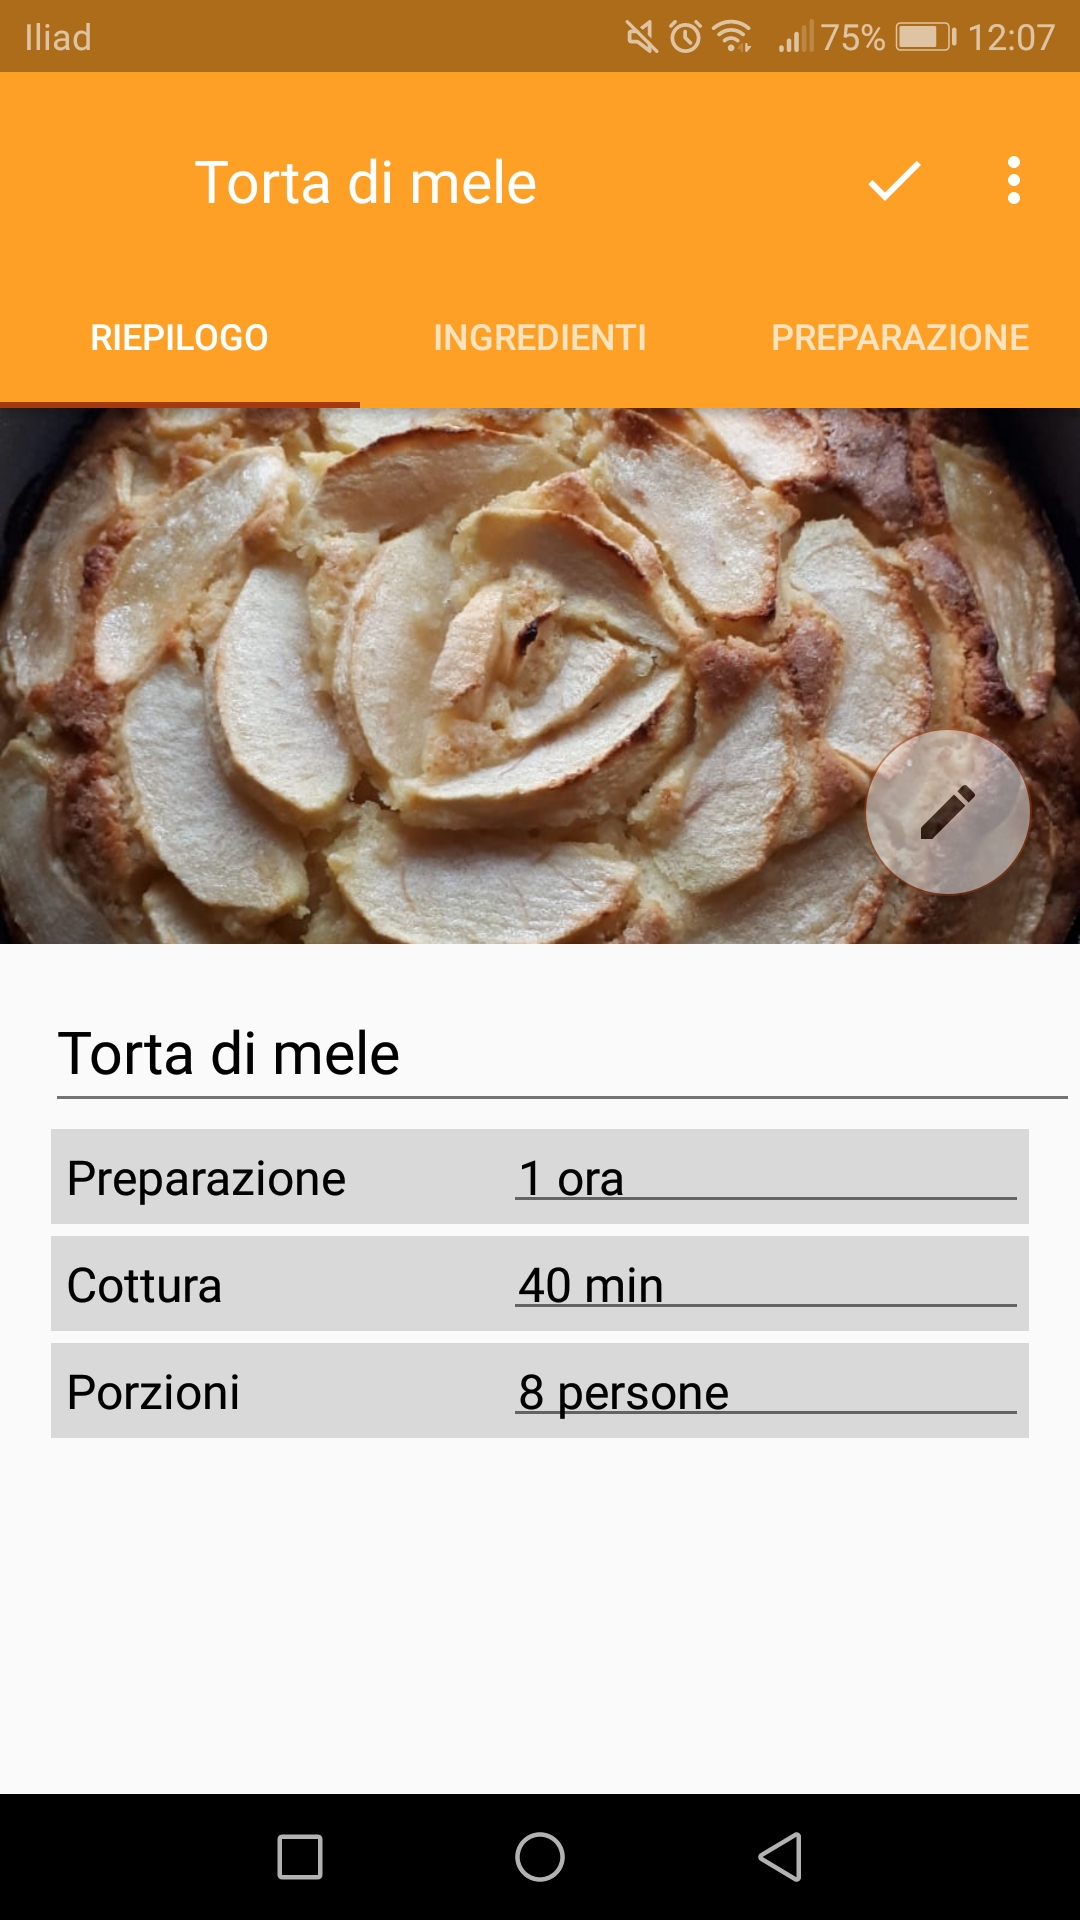
\includegraphics[width=0.49\textwidth]{definitivo/edit_riepilogo}
    \caption{Azione di condivisione e modifica del riepilogo}
    \label{fig:def_ricetta_2}
  \end{center}
\end{figure}

\begin{figure}[ht]
  \begin{center}
    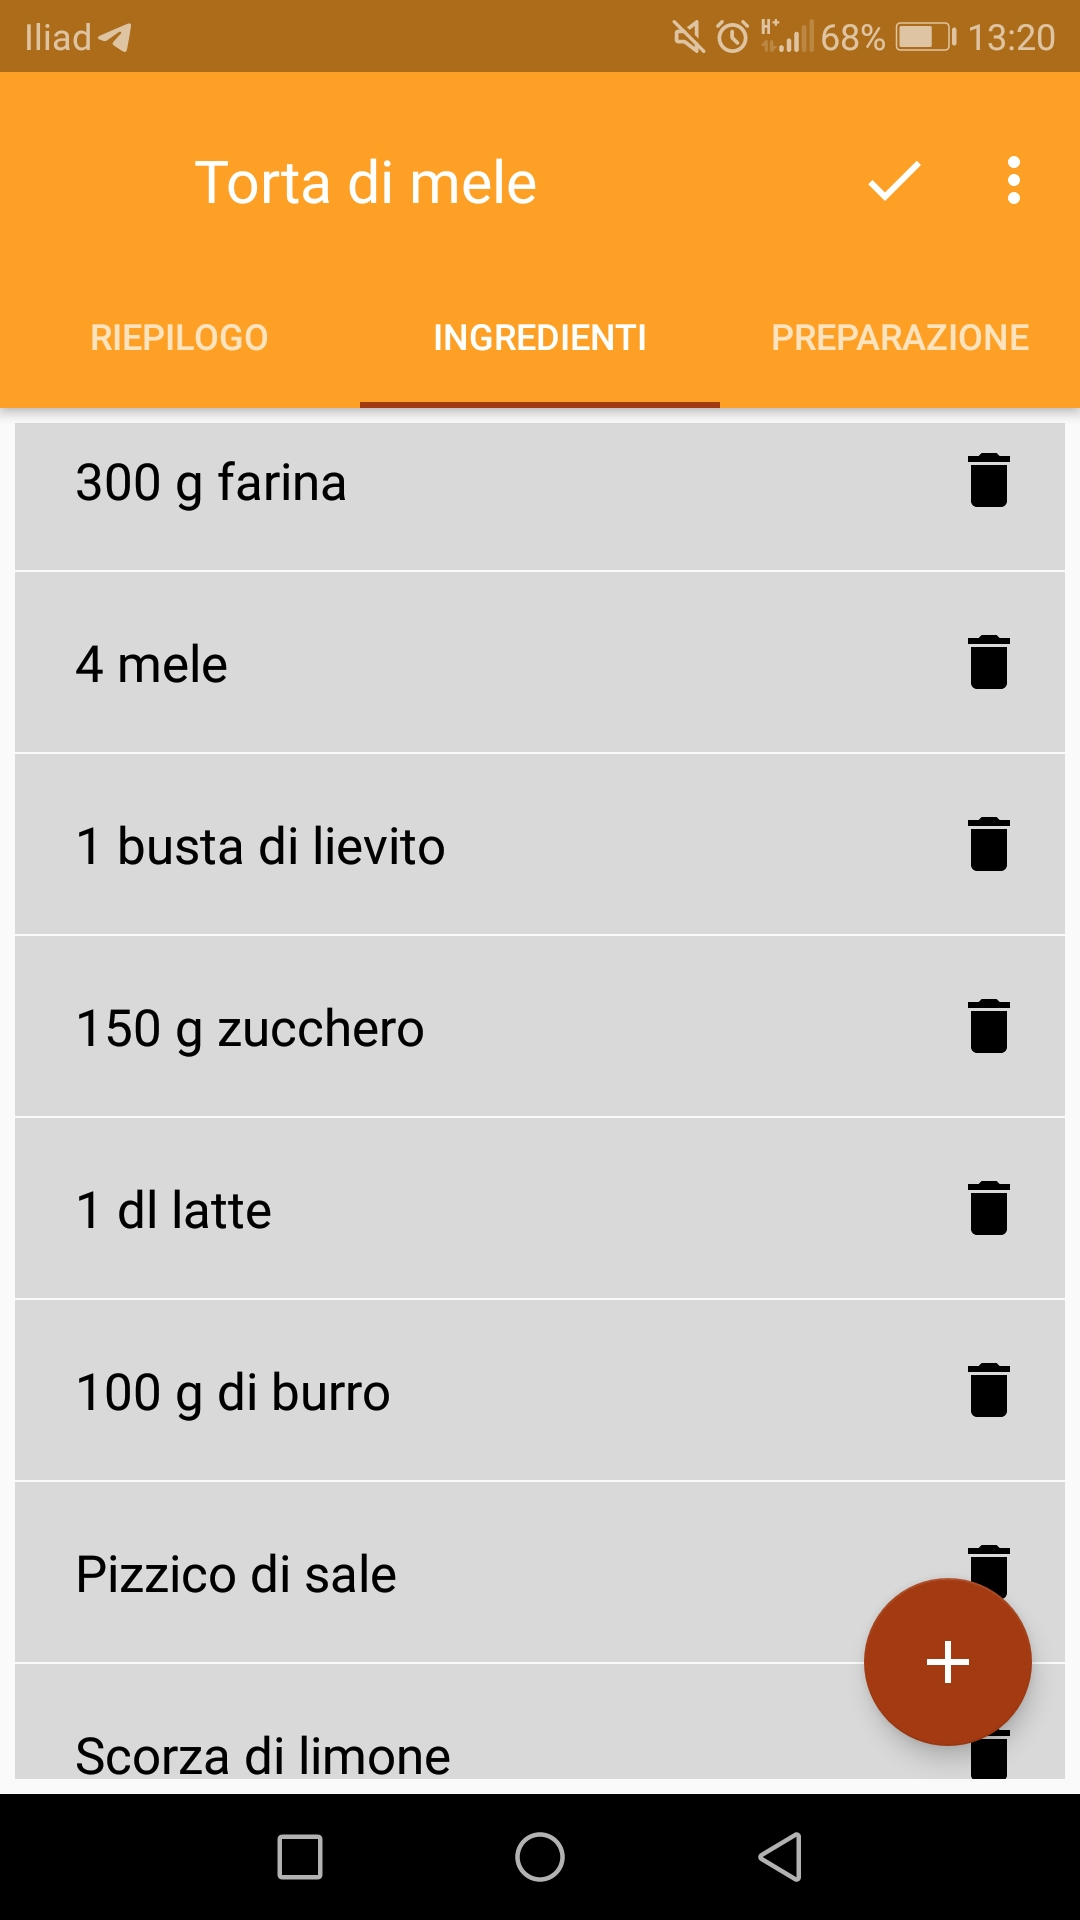
\includegraphics[width=0.49\textwidth]{definitivo/edit_ingredienti}
    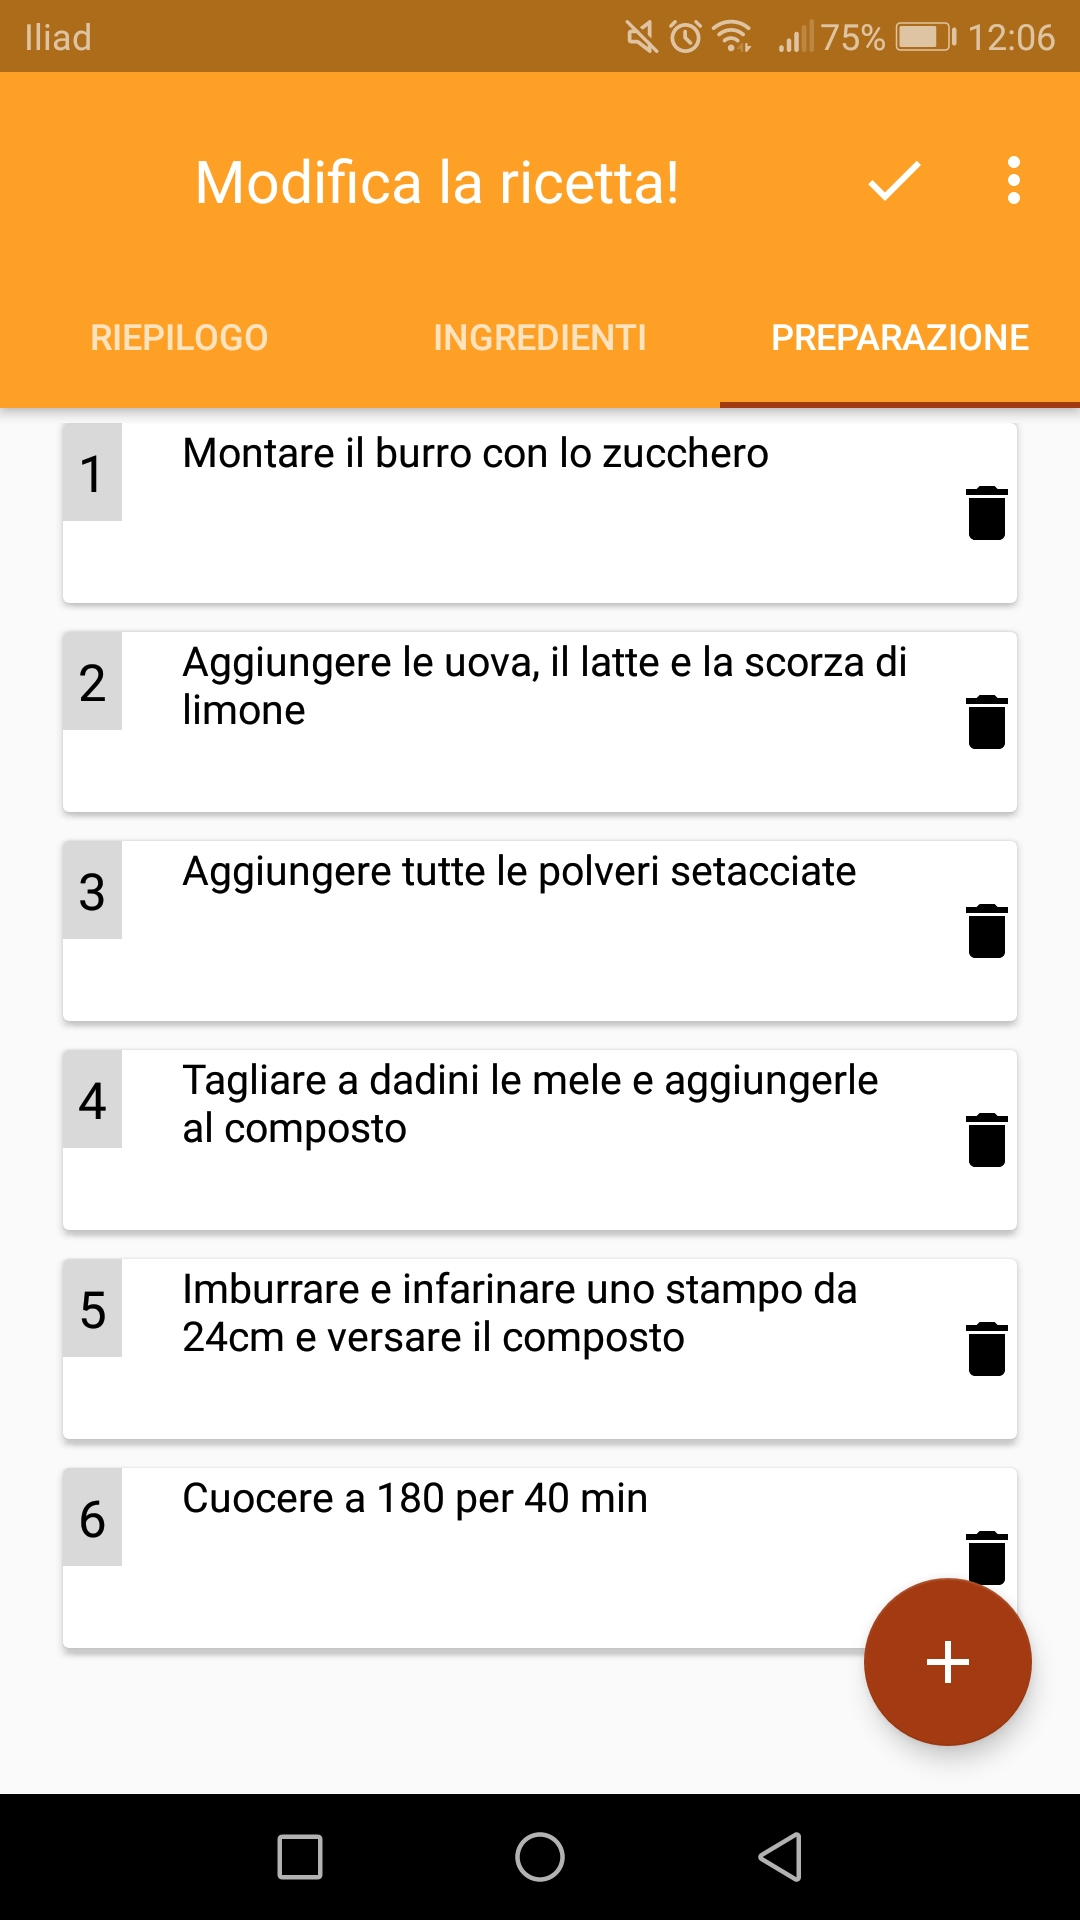
\includegraphics[width=0.49\textwidth]{definitivo/edit_preparazione}
    \caption{Modifica degli ingredienti e dei passaggi}
    \label{fig:def_edit_ricetta}
  \end{center}
\end{figure}

\begin{figure}[ht]
  \begin{center}
    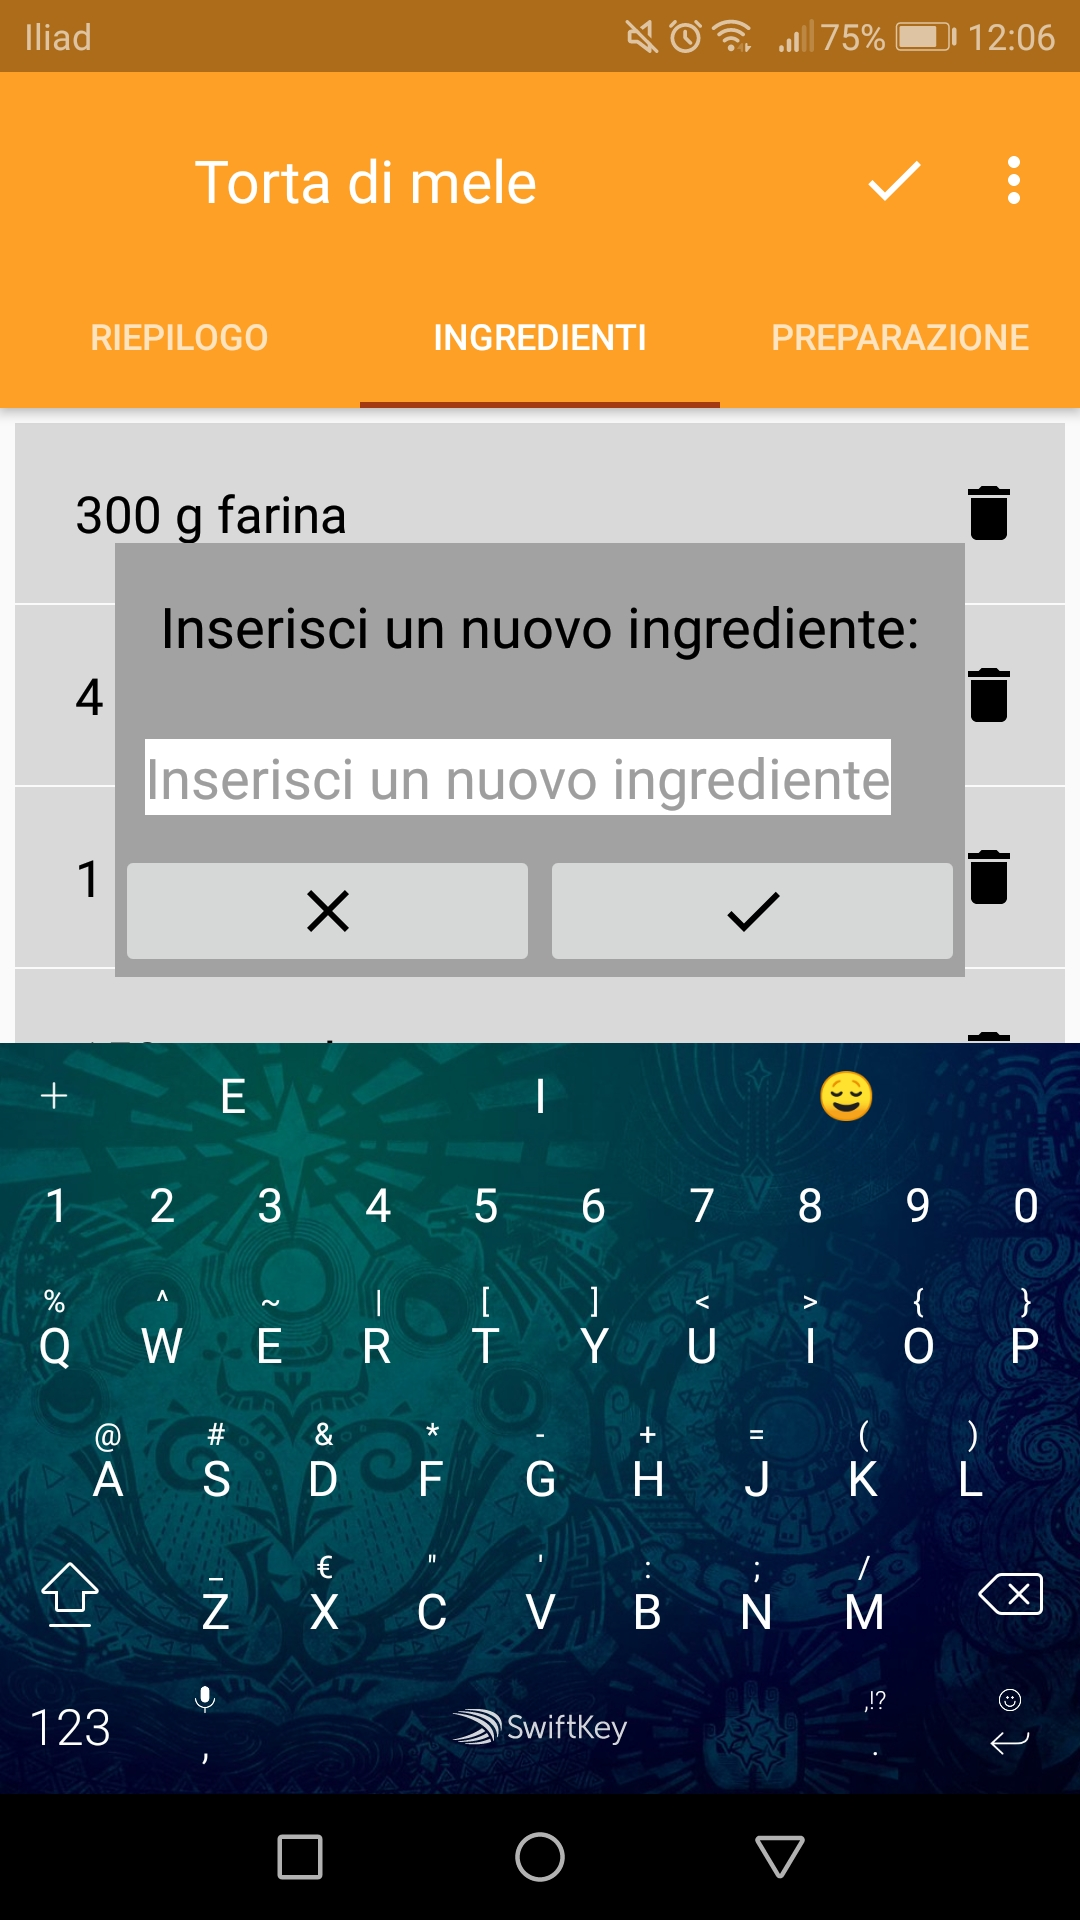
\includegraphics[width=0.49\textwidth]{definitivo/add_ingrediente}
    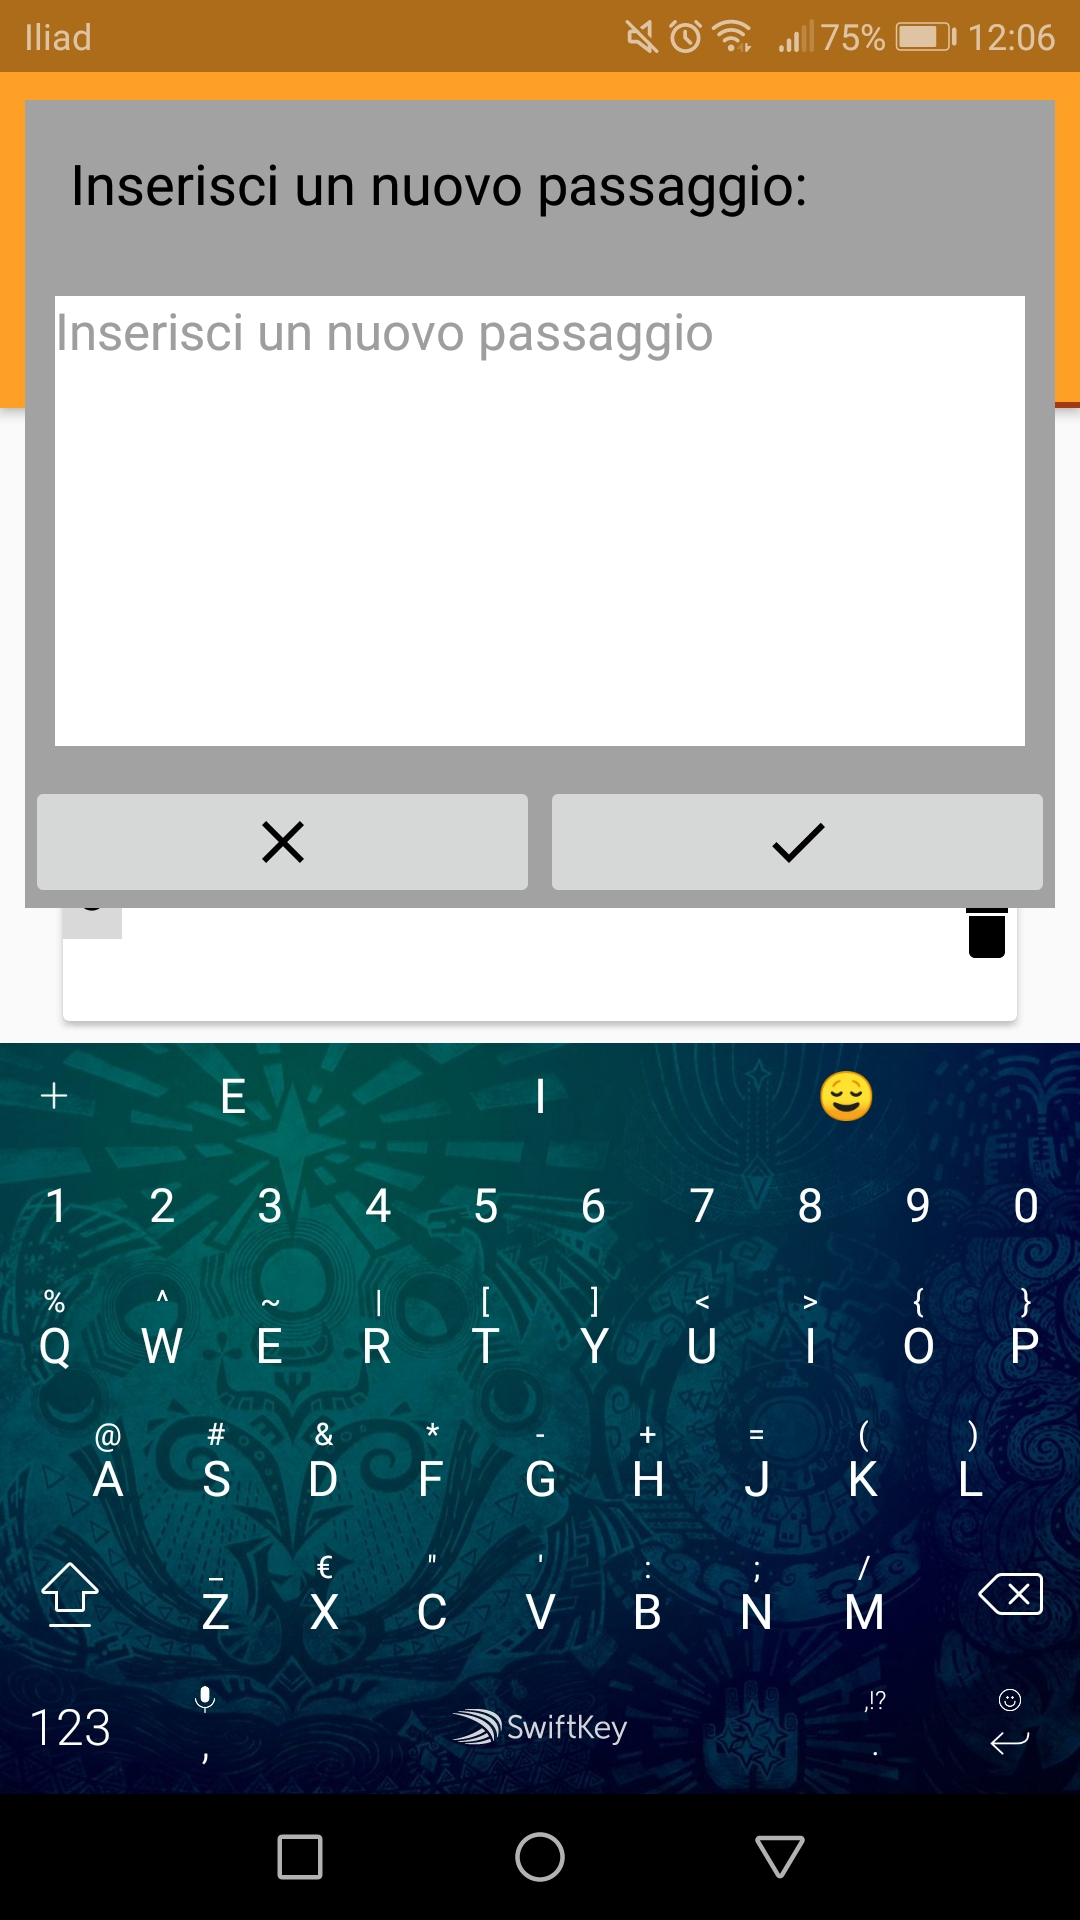
\includegraphics[width=0.49\textwidth]{definitivo/add_step}
    \caption{Finestre di aggiunta ingrediente e passaggio}
    \label{fig:def_edit_ricetta_1}
  \end{center}
\end{figure}

\clearpage
\subsection{Differenze dalla progettazione}
Nella schermata di riepilogo, nonostante il database delle ricette sia già predisposto, non vengono visualizzate difficoltà e tags.
Inoltre non è stata implementata l'attività dell'assistente.
Queste scelte sono state fatte per concentrare l'attenzione sulle schermate e sulle funzionalità principali.
Si è preferito analizzare con maggior cura le attività principali piuttosto che aggiungerne altre ed introdurre errori o gravi bachi.
I TAG non sono stati aggiunti perché la loro utilità risiedeva nel poter essere condivisi fra più ricette, in modo da poterle eventualmente partizionare per TAG.
Di nuovo, si è preferito evitare di aggiungere ulteriore complessità.

\subsection{Problematiche Principali}
Tralasciando problematiche banali o dovute al fatto che questo è il risultato di un primo approccio allo strumento \textit{Android Studio}, una delle difficoltà principali riguarda gli \textit{ImageView}.
Quando l'utente seleziona l'immagine, questa viene caricata correttamente sia nella schermata di riepilogo che nel \textit{ViewHolder} del \textit{RecyclerView} delle ricette. 
Purtroppo gli \textit{ImageView} si comportano in modi inaspettati quando si cambia attività, ma soprattutto quando viene selezionata la stessa immagine più volte.
Nonostante sia stato investito parecchio tempo alla ricerca di una soluzione, non è stato possibile trovarne nessuna soddisfacente.
Seguendo i numerosi consigli trovati in rete, il problema persiste.

In fase di consegna del progetto avrei potuto omettere tutto ciò che riguardava le immagini ma, anche se \textit{feature} incompleta, ho preferito lasciarlo.
Principalmente per dar valore al tempo speso alla ricerca di una soluzione ed in secondo luogo perché in ogni sito o libro di ricette vengono illustrate le foto dei risultati.

\begin{figure}[ht]
  \begin{center}
    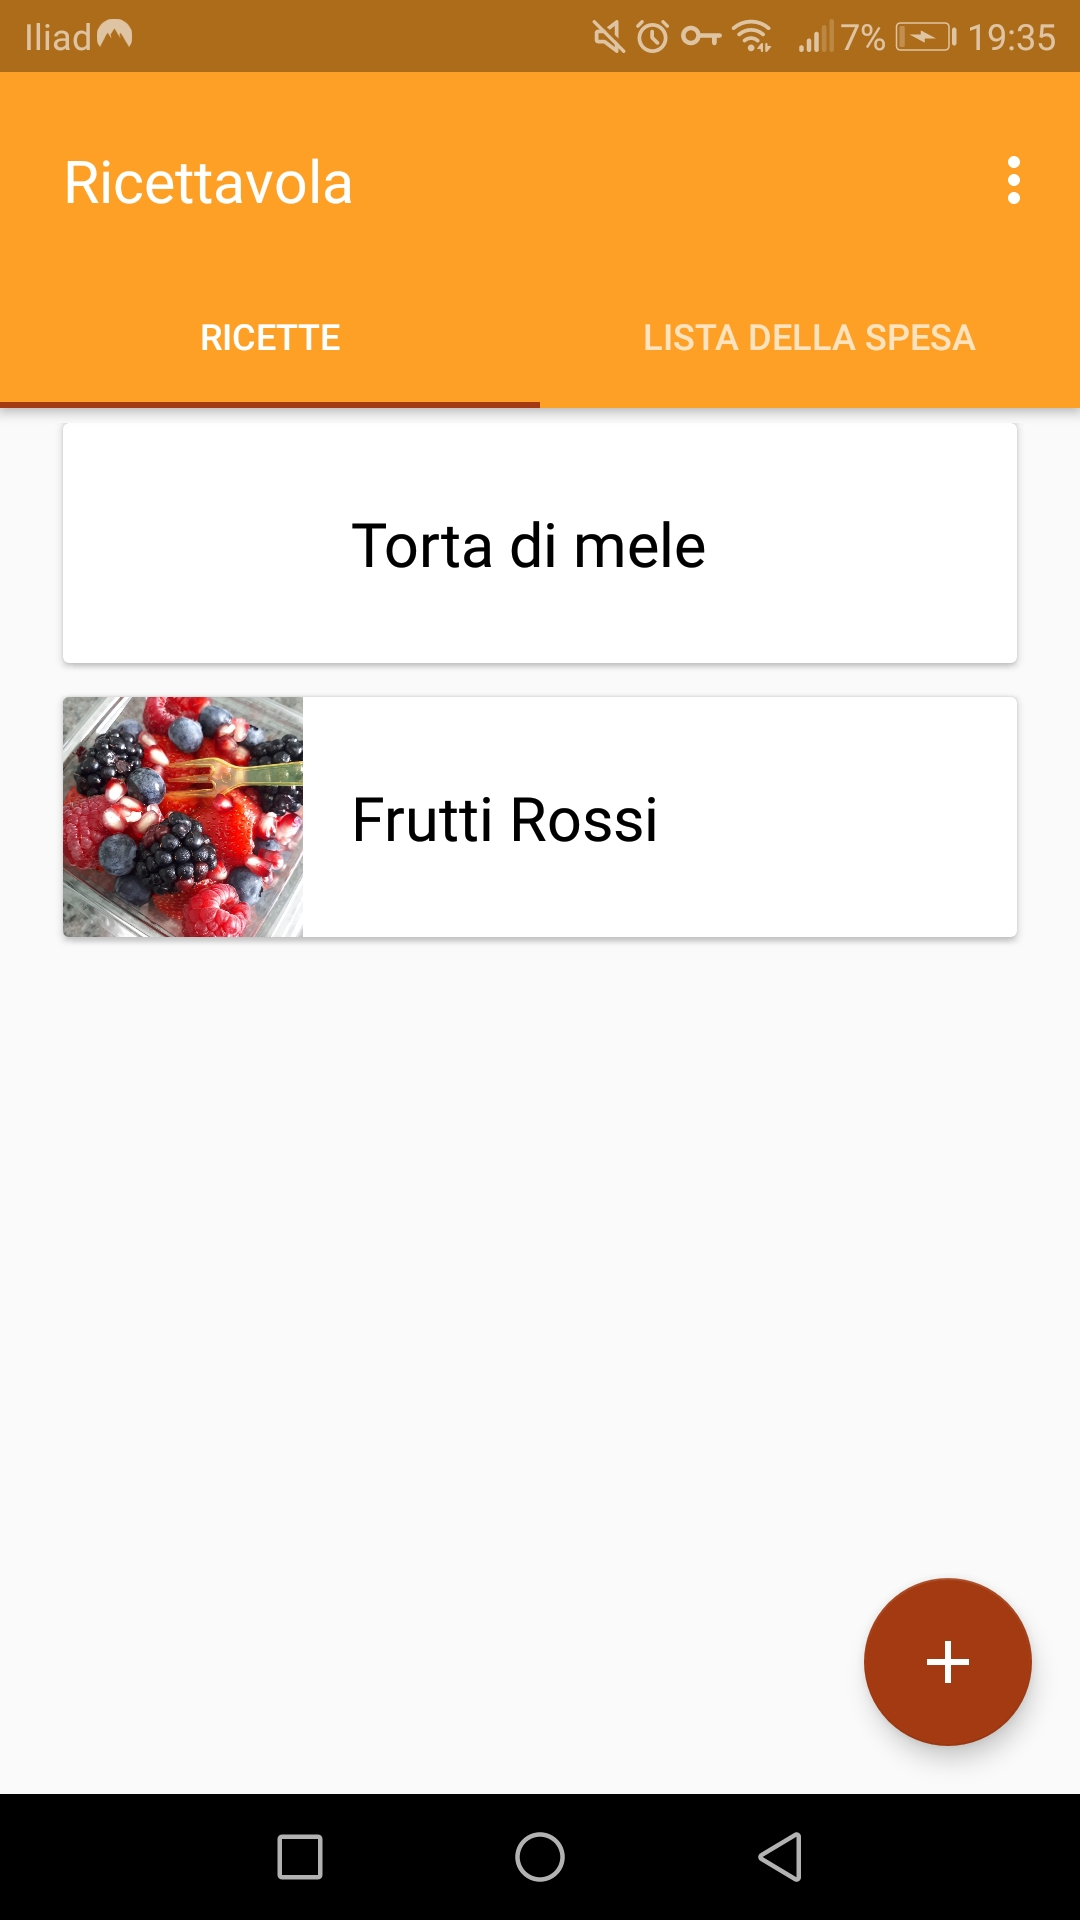
\includegraphics[width=0.49\textwidth]{definitivo/bug_1}
    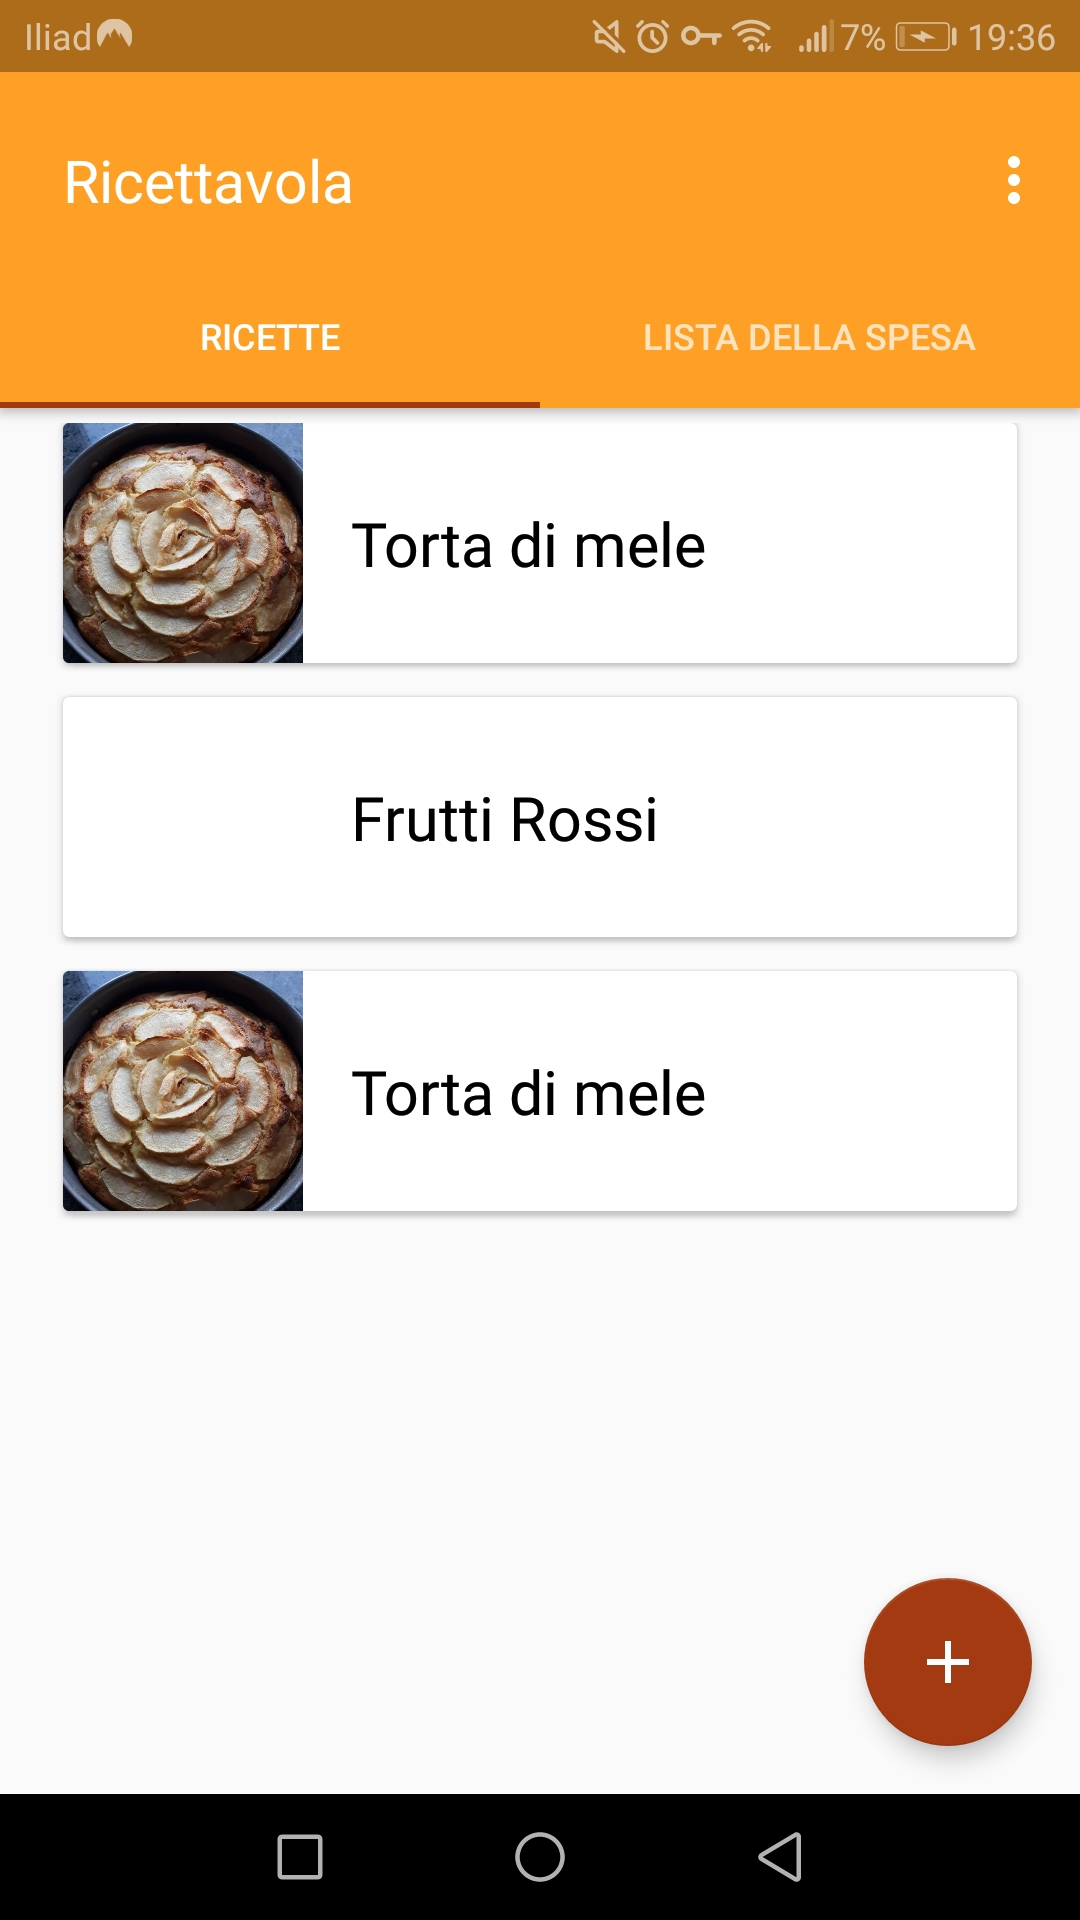
\includegraphics[width=0.49\textwidth]{definitivo/bug_2}
    \caption{Dimostrazione dei comportamenti particolari degli ImageView}
    \label{fig:bug_1}
  \end{center}
\end{figure}

In figura \ref{fig:bug_1} ed in figura \ref{fig:bug_2} sono riportate le schermate che mostrano la problematica.
La prima schermata in figura \ref{fig:bug_1} contiene due ricette: la prima dovrebbe mostrare la foto di una torta alle mele, la seconda viene mostrata correttamente.
Nella seconda schermata è state creata una copia della ricetta alle mele (utilizzando la funzionalità di esportazione ed importazione tramite \textit{clipboard}), associando a questa nuova copia la stessa immagine di prima, ci si accorge che ogni occorrenza dell'immagine viene mostrata correttamente.
In figura \ref{fig:bug_2} è stato effettuata la stessa procedura ma con l'immagine dei frutti.

Si supponeva che tale comportamento fosse dovuto al modo in cui si ottengono i riferimenti alle immagini, ma anche utilizzando chiamate ad altre attività differenti ("applicazione galleria" piuttosto che applicazione "foto" oppure "galleria di Google").
Si è provato ad usare \textit{ImageView} differenti oppure a segnalarli come invalidi, ma nulla ha risolto questa problematica.


\begin{figure}[ht]
  \begin{center}
    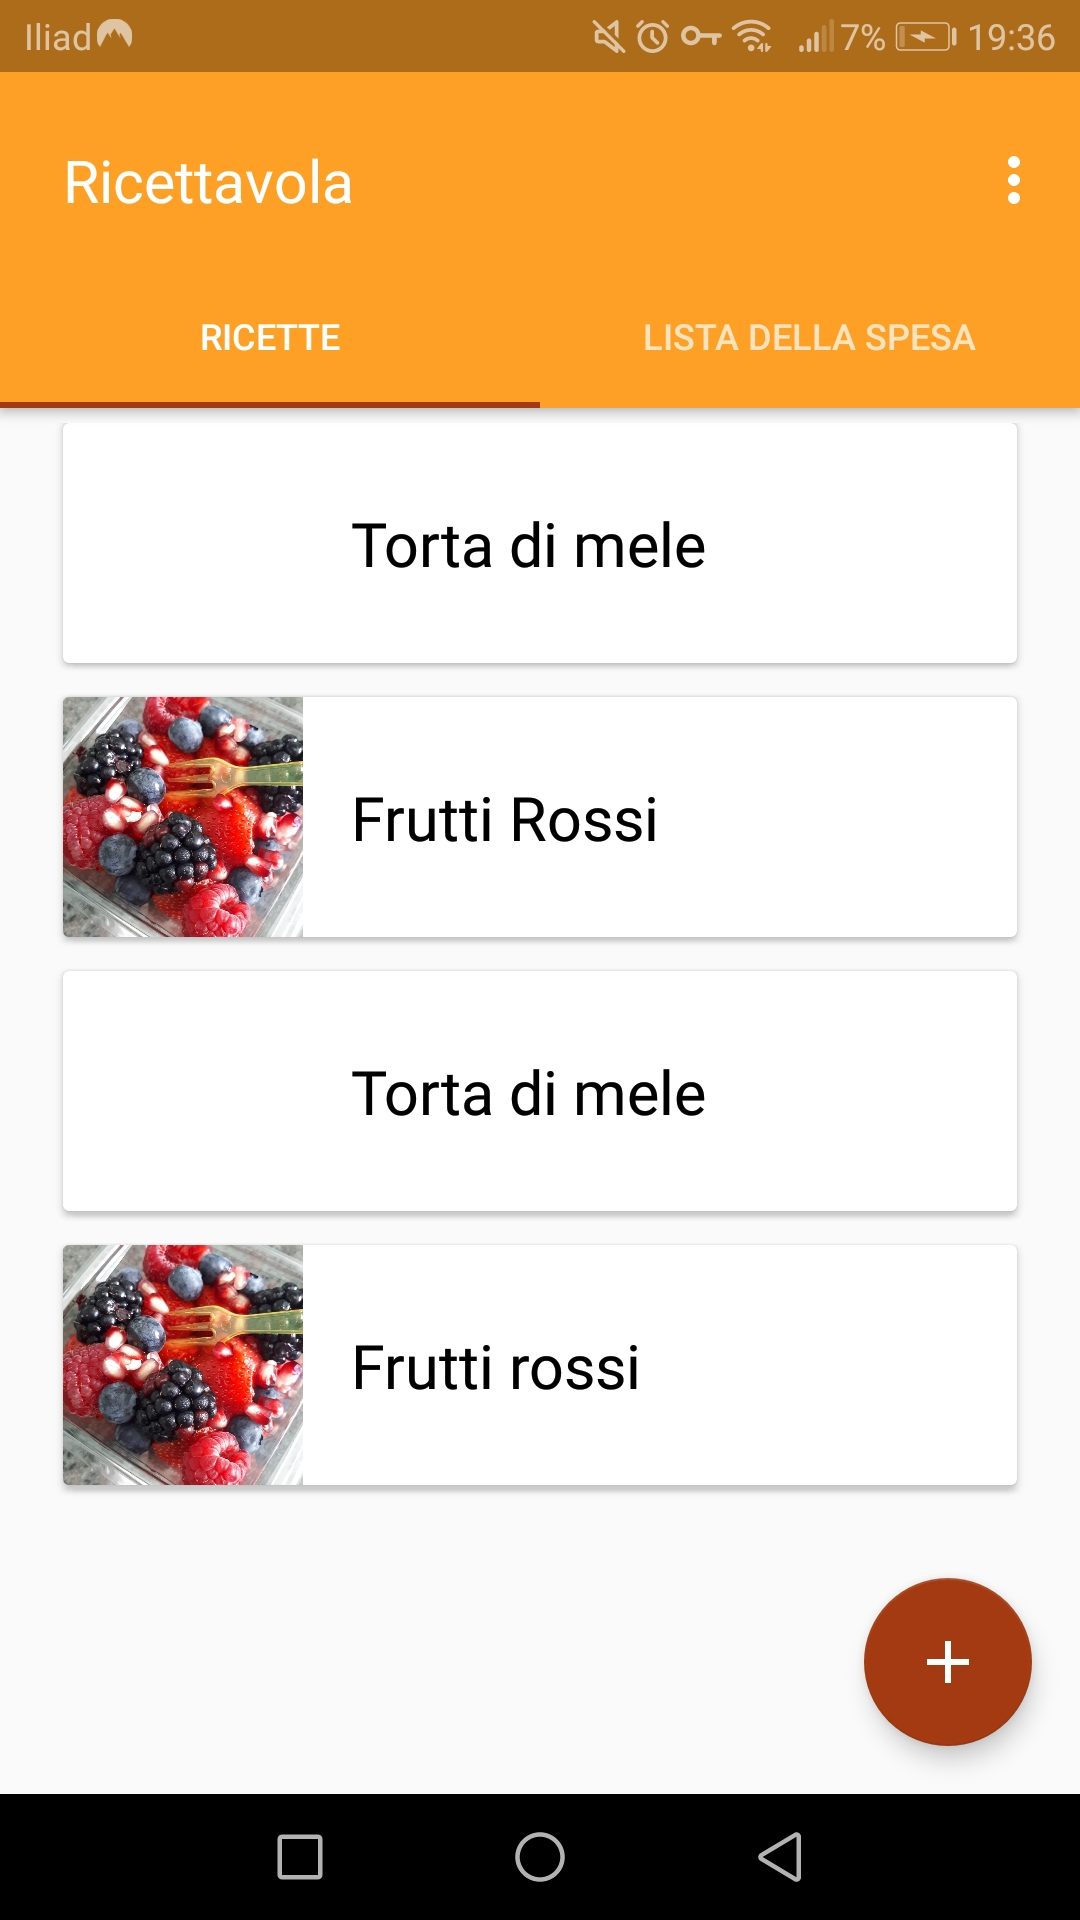
\includegraphics[width=0.49\textwidth]{definitivo/bug_3}
    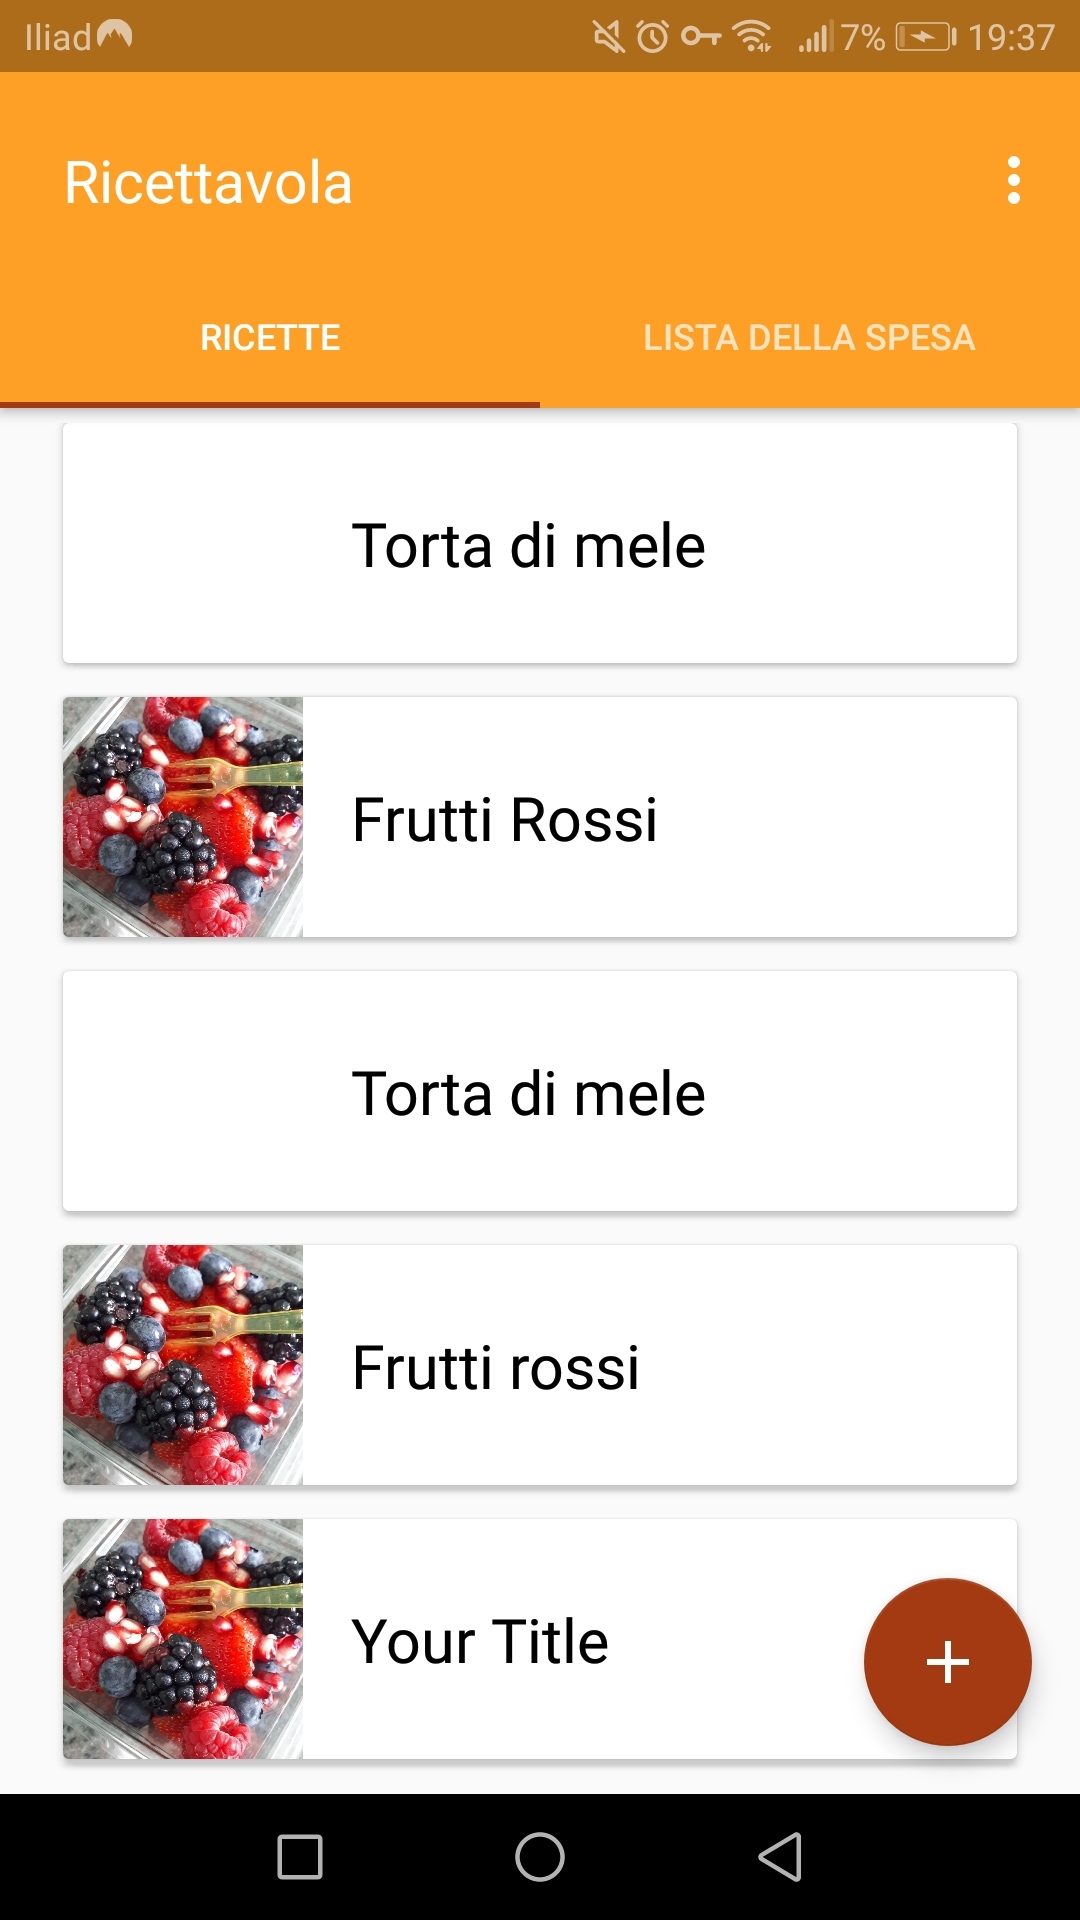
\includegraphics[width=0.49\textwidth]{definitivo/bug_4}
    \caption{Dimostrazione dei comportamenti particolari degli ImageView}
    \label{fig:bug_2}
  \end{center}
\end{figure}

